\documentclass{llncs}
\usepackage{hyperref}
\usepackage{url}
\pagestyle{plain}
\usepackage{threeparttable}
%%%%% NEW MATH DEFINITIONS %%%%%

\usepackage{amsmath,amsfonts,bm}

% Mark sections of captions for referring to divisions of figures
\newcommand{\figleft}{{\em (Left)}}
\newcommand{\figcenter}{{\em (Center)}}
\newcommand{\figright}{{\em (Right)}}
\newcommand{\figtop}{{\em (Top)}}
\newcommand{\figbottom}{{\em (Bottom)}}
\newcommand{\captiona}{{\em (a)}}
\newcommand{\captionb}{{\em (b)}}
\newcommand{\captionc}{{\em (c)}}
\newcommand{\captiond}{{\em (d)}}

% Highlight a newly defined term
\newcommand{\newterm}[1]{{\bf #1}}


% Figure reference, lower-case.
\def\figref#1{figure~\ref{#1}}
% Figure reference, capital. For start of sentence
\def\Figref#1{Figure~\ref{#1}}
\def\twofigref#1#2{figures \ref{#1} and \ref{#2}}
\def\quadfigref#1#2#3#4{figures \ref{#1}, \ref{#2}, \ref{#3} and \ref{#4}}
% Section reference, lower-case.
\def\secref#1{section~\ref{#1}}
% Section reference, capital.
\def\Secref#1{Section~\ref{#1}}
% Reference to two sections.
\def\twosecrefs#1#2{sections \ref{#1} and \ref{#2}}
% Reference to three sections.
\def\secrefs#1#2#3{sections \ref{#1}, \ref{#2} and \ref{#3}}
% Reference to an equation, lower-case.
\def\eqref#1{equation~\ref{#1}}
% Reference to an equation, upper case
\def\Eqref#1{Equation~\ref{#1}}
% A raw reference to an equation---avoid using if possible
\def\plaineqref#1{\ref{#1}}
% Reference to a chapter, lower-case.
\def\chapref#1{chapter~\ref{#1}}
% Reference to an equation, upper case.
\def\Chapref#1{Chapter~\ref{#1}}
% Reference to a range of chapters
\def\rangechapref#1#2{chapters\ref{#1}--\ref{#2}}
% Reference to an algorithm, lower-case.
\def\algref#1{algorithm~\ref{#1}}
% Reference to an algorithm, upper case.
\def\Algref#1{Algorithm~\ref{#1}}
\def\twoalgref#1#2{algorithms \ref{#1} and \ref{#2}}
\def\Twoalgref#1#2{Algorithms \ref{#1} and \ref{#2}}
% Reference to a part, lower case
\def\partref#1{part~\ref{#1}}
% Reference to a part, upper case
\def\Partref#1{Part~\ref{#1}}
\def\twopartref#1#2{parts \ref{#1} and \ref{#2}}

\def\ceil#1{\lceil #1 \rceil}
\def\floor#1{\lfloor #1 \rfloor}
\def\1{\bm{1}}
\newcommand{\train}{\mathcal{D}}
\newcommand{\valid}{\mathcal{D_{\mathrm{valid}}}}
\newcommand{\test}{\mathcal{D_{\mathrm{test}}}}

\def\eps{{\epsilon}}


% Random variables
\def\reta{{\textnormal{$\eta$}}}
\def\ra{{\textnormal{a}}}
\def\rb{{\textnormal{b}}}
\def\rc{{\textnormal{c}}}
\def\rd{{\textnormal{d}}}
\def\re{{\textnormal{e}}}
\def\rf{{\textnormal{f}}}
\def\rg{{\textnormal{g}}}
\def\rh{{\textnormal{h}}}
\def\ri{{\textnormal{i}}}
\def\rj{{\textnormal{j}}}
\def\rk{{\textnormal{k}}}
\def\rl{{\textnormal{l}}}
% rm is already a command, just don't name any random variables m
\def\rn{{\textnormal{n}}}
\def\ro{{\textnormal{o}}}
\def\rp{{\textnormal{p}}}
\def\rq{{\textnormal{q}}}
\def\rr{{\textnormal{r}}}
\def\rs{{\textnormal{s}}}
\def\rt{{\textnormal{t}}}
\def\ru{{\textnormal{u}}}
\def\rv{{\textnormal{v}}}
\def\rw{{\textnormal{w}}}
\def\rx{{\textnormal{x}}}
\def\ry{{\textnormal{y}}}
\def\rz{{\textnormal{z}}}

% Random vectors
\def\rvepsilon{{\mathbf{\epsilon}}}
\def\rvtheta{{\mathbf{\theta}}}
\def\rva{{\mathbf{a}}}
\def\rvb{{\mathbf{b}}}
\def\rvc{{\mathbf{c}}}
\def\rvd{{\mathbf{d}}}
\def\rve{{\mathbf{e}}}
\def\rvf{{\mathbf{f}}}
\def\rvg{{\mathbf{g}}}
\def\rvh{{\mathbf{h}}}
\def\rvu{{\mathbf{i}}}
\def\rvj{{\mathbf{j}}}
\def\rvk{{\mathbf{k}}}
\def\rvl{{\mathbf{l}}}
\def\rvm{{\mathbf{m}}}
\def\rvn{{\mathbf{n}}}
\def\rvo{{\mathbf{o}}}
\def\rvp{{\mathbf{p}}}
\def\rvq{{\mathbf{q}}}
\def\rvr{{\mathbf{r}}}
\def\rvs{{\mathbf{s}}}
\def\rvt{{\mathbf{t}}}
\def\rvu{{\mathbf{u}}}
\def\rvv{{\mathbf{v}}}
\def\rvw{{\mathbf{w}}}
\def\rvx{{\mathbf{x}}}
\def\rvy{{\mathbf{y}}}
\def\rvz{{\mathbf{z}}}

% Elements of random vectors
\def\erva{{\textnormal{a}}}
\def\ervb{{\textnormal{b}}}
\def\ervc{{\textnormal{c}}}
\def\ervd{{\textnormal{d}}}
\def\erve{{\textnormal{e}}}
\def\ervf{{\textnormal{f}}}
\def\ervg{{\textnormal{g}}}
\def\ervh{{\textnormal{h}}}
\def\ervi{{\textnormal{i}}}
\def\ervj{{\textnormal{j}}}
\def\ervk{{\textnormal{k}}}
\def\ervl{{\textnormal{l}}}
\def\ervm{{\textnormal{m}}}
\def\ervn{{\textnormal{n}}}
\def\ervo{{\textnormal{o}}}
\def\ervp{{\textnormal{p}}}
\def\ervq{{\textnormal{q}}}
\def\ervr{{\textnormal{r}}}
\def\ervs{{\textnormal{s}}}
\def\ervt{{\textnormal{t}}}
\def\ervu{{\textnormal{u}}}
\def\ervv{{\textnormal{v}}}
\def\ervw{{\textnormal{w}}}
\def\ervx{{\textnormal{x}}}
\def\ervy{{\textnormal{y}}}
\def\ervz{{\textnormal{z}}}

% Random matrices
\def\rmA{{\mathbf{A}}}
\def\rmB{{\mathbf{B}}}
\def\rmC{{\mathbf{C}}}
\def\rmD{{\mathbf{D}}}
\def\rmE{{\mathbf{E}}}
\def\rmF{{\mathbf{F}}}
\def\rmG{{\mathbf{G}}}
\def\rmH{{\mathbf{H}}}
\def\rmI{{\mathbf{I}}}
\def\rmJ{{\mathbf{J}}}
\def\rmK{{\mathbf{K}}}
\def\rmL{{\mathbf{L}}}
\def\rmM{{\mathbf{M}}}
\def\rmN{{\mathbf{N}}}
\def\rmO{{\mathbf{O}}}
\def\rmP{{\mathbf{P}}}
\def\rmQ{{\mathbf{Q}}}
\def\rmR{{\mathbf{R}}}
\def\rmS{{\mathbf{S}}}
\def\rmT{{\mathbf{T}}}
\def\rmU{{\mathbf{U}}}
\def\rmV{{\mathbf{V}}}
\def\rmW{{\mathbf{W}}}
\def\rmX{{\mathbf{X}}}
\def\rmY{{\mathbf{Y}}}
\def\rmZ{{\mathbf{Z}}}

% Elements of random matrices
\def\ermA{{\textnormal{A}}}
\def\ermB{{\textnormal{B}}}
\def\ermC{{\textnormal{C}}}
\def\ermD{{\textnormal{D}}}
\def\ermE{{\textnormal{E}}}
\def\ermF{{\textnormal{F}}}
\def\ermG{{\textnormal{G}}}
\def\ermH{{\textnormal{H}}}
\def\ermI{{\textnormal{I}}}
\def\ermJ{{\textnormal{J}}}
\def\ermK{{\textnormal{K}}}
\def\ermL{{\textnormal{L}}}
\def\ermM{{\textnormal{M}}}
\def\ermN{{\textnormal{N}}}
\def\ermO{{\textnormal{O}}}
\def\ermP{{\textnormal{P}}}
\def\ermQ{{\textnormal{Q}}}
\def\ermR{{\textnormal{R}}}
\def\ermS{{\textnormal{S}}}
\def\ermT{{\textnormal{T}}}
\def\ermU{{\textnormal{U}}}
\def\ermV{{\textnormal{V}}}
\def\ermW{{\textnormal{W}}}
\def\ermX{{\textnormal{X}}}
\def\ermY{{\textnormal{Y}}}
\def\ermZ{{\textnormal{Z}}}

% Vectors
\def\vzero{{\bm{0}}}
\def\vone{{\bm{1}}}
\def\vmu{{\bm{\mu}}}
\def\vtheta{{\bm{\theta}}}
\def\va{{\bm{a}}}
\def\vb{{\bm{b}}}
\def\vc{{\bm{c}}}
\def\vd{{\bm{d}}}
\def\ve{{\bm{e}}}
\def\vf{{\bm{f}}}
\def\vg{{\bm{g}}}
\def\vh{{\bm{h}}}
\def\vi{{\bm{i}}}
\def\vj{{\bm{j}}}
\def\vk{{\bm{k}}}
\def\vl{{\bm{l}}}
\def\vm{{\bm{m}}}
\def\vn{{\bm{n}}}
\def\vo{{\bm{o}}}
\def\vp{{\bm{p}}}
\def\vq{{\bm{q}}}
\def\vr{{\bm{r}}}
\def\vs{{\bm{s}}}
\def\vt{{\bm{t}}}
\def\vu{{\bm{u}}}
\def\vv{{\bm{v}}}
\def\vw{{\bm{w}}}
\def\vx{{\bm{x}}}
\def\vy{{\bm{y}}}
\def\vz{{\bm{z}}}

% Elements of vectors
\def\evalpha{{\alpha}}
\def\evbeta{{\beta}}
\def\evepsilon{{\epsilon}}
\def\evlambda{{\lambda}}
\def\evomega{{\omega}}
\def\evmu{{\mu}}
\def\evpsi{{\psi}}
\def\evsigma{{\sigma}}
\def\evtheta{{\theta}}
\def\eva{{a}}
\def\evb{{b}}
\def\evc{{c}}
\def\evd{{d}}
\def\eve{{e}}
\def\evf{{f}}
\def\evg{{g}}
\def\evh{{h}}
\def\evi{{i}}
\def\evj{{j}}
\def\evk{{k}}
\def\evl{{l}}
\def\evm{{m}}
\def\evn{{n}}
\def\evo{{o}}
\def\evp{{p}}
\def\evq{{q}}
\def\evr{{r}}
\def\evs{{s}}
\def\evt{{t}}
\def\evu{{u}}
\def\evv{{v}}
\def\evw{{w}}
\def\evx{{x}}
\def\evy{{y}}
\def\evz{{z}}

% Matrix
\def\mA{{\bm{A}}}
\def\mB{{\bm{B}}}
\def\mC{{\bm{C}}}
\def\mD{{\bm{D}}}
\def\mE{{\bm{E}}}
\def\mF{{\bm{F}}}
\def\mG{{\bm{G}}}
\def\mH{{\bm{H}}}
\def\mI{{\bm{I}}}
\def\mJ{{\bm{J}}}
\def\mK{{\bm{K}}}
\def\mL{{\bm{L}}}
\def\mM{{\bm{M}}}
\def\mN{{\bm{N}}}
\def\mO{{\bm{O}}}
\def\mP{{\bm{P}}}
\def\mQ{{\bm{Q}}}
\def\mR{{\bm{R}}}
\def\mS{{\bm{S}}}
\def\mT{{\bm{T}}}
\def\mU{{\bm{U}}}
\def\mV{{\bm{V}}}
\def\mW{{\bm{W}}}
\def\mX{{\bm{X}}}
\def\mY{{\bm{Y}}}
\def\mZ{{\bm{Z}}}
\def\mBeta{{\bm{\beta}}}
\def\mPhi{{\bm{\Phi}}}
\def\mLambda{{\bm{\Lambda}}}
\def\mSigma{{\bm{\Sigma}}}

% Tensor
\DeclareMathAlphabet{\mathsfit}{\encodingdefault}{\sfdefault}{m}{sl}
\SetMathAlphabet{\mathsfit}{bold}{\encodingdefault}{\sfdefault}{bx}{n}
\newcommand{\tens}[1]{\bm{\mathsfit{#1}}}
\def\tA{{\tens{A}}}
\def\tB{{\tens{B}}}
\def\tC{{\tens{C}}}
\def\tD{{\tens{D}}}
\def\tE{{\tens{E}}}
\def\tF{{\tens{F}}}
\def\tG{{\tens{G}}}
\def\tH{{\tens{H}}}
\def\tI{{\tens{I}}}
\def\tJ{{\tens{J}}}
\def\tK{{\tens{K}}}
\def\tL{{\tens{L}}}
\def\tM{{\tens{M}}}
\def\tN{{\tens{N}}}
\def\tO{{\tens{O}}}
\def\tP{{\tens{P}}}
\def\tQ{{\tens{Q}}}
\def\tR{{\tens{R}}}
\def\tS{{\tens{S}}}
\def\tT{{\tens{T}}}
\def\tU{{\tens{U}}}
\def\tV{{\tens{V}}}
\def\tW{{\tens{W}}}
\def\tX{{\tens{X}}}
\def\tY{{\tens{Y}}}
\def\tZ{{\tens{Z}}}


% Graph
\def\gA{{\mathcal{A}}}
\def\gB{{\mathcal{B}}}
\def\gC{{\mathcal{C}}}
\def\gD{{\mathcal{D}}}
\def\gE{{\mathcal{E}}}
\def\gF{{\mathcal{F}}}
\def\gG{{\mathcal{G}}}
\def\gH{{\mathcal{H}}}
\def\gI{{\mathcal{I}}}
\def\gJ{{\mathcal{J}}}
\def\gK{{\mathcal{K}}}
\def\gL{{\mathcal{L}}}
\def\gM{{\mathcal{M}}}
\def\gN{{\mathcal{N}}}
\def\gO{{\mathcal{O}}}
\def\gP{{\mathcal{P}}}
\def\gQ{{\mathcal{Q}}}
\def\gR{{\mathcal{R}}}
\def\gS{{\mathcal{S}}}
\def\gT{{\mathcal{T}}}
\def\gU{{\mathcal{U}}}
\def\gV{{\mathcal{V}}}
\def\gW{{\mathcal{W}}}
\def\gX{{\mathcal{X}}}
\def\gY{{\mathcal{Y}}}
\def\gZ{{\mathcal{Z}}}

% Sets
\def\sA{{\mathbb{A}}}
\def\sB{{\mathbb{B}}}
\def\sC{{\mathbb{C}}}
\def\sD{{\mathbb{D}}}
% Don't use a set called E, because this would be the same as our symbol
% for expectation.
\def\sF{{\mathbb{F}}}
\def\sG{{\mathbb{G}}}
\def\sH{{\mathbb{H}}}
\def\sI{{\mathbb{I}}}
\def\sJ{{\mathbb{J}}}
\def\sK{{\mathbb{K}}}
\def\sL{{\mathbb{L}}}
\def\sM{{\mathbb{M}}}
\def\sN{{\mathbb{N}}}
\def\sO{{\mathbb{O}}}
\def\sP{{\mathbb{P}}}
\def\sQ{{\mathbb{Q}}}
\def\sR{{\mathbb{R}}}
\def\sS{{\mathbb{S}}}
\def\sT{{\mathbb{T}}}
\def\sU{{\mathbb{U}}}
\def\sV{{\mathbb{V}}}
\def\sW{{\mathbb{W}}}
\def\sX{{\mathbb{X}}}
\def\sY{{\mathbb{Y}}}
\def\sZ{{\mathbb{Z}}}

% Entries of a matrix
\def\emLambda{{\Lambda}}
\def\emA{{A}}
\def\emB{{B}}
\def\emC{{C}}
\def\emD{{D}}
\def\emE{{E}}
\def\emF{{F}}
\def\emG{{G}}
\def\emH{{H}}
\def\emI{{I}}
\def\emJ{{J}}
\def\emK{{K}}
\def\emL{{L}}
\def\emM{{M}}
\def\emN{{N}}
\def\emO{{O}}
\def\emP{{P}}
\def\emQ{{Q}}
\def\emR{{R}}
\def\emS{{S}}
\def\emT{{T}}
\def\emU{{U}}
\def\emV{{V}}
\def\emW{{W}}
\def\emX{{X}}
\def\emY{{Y}}
\def\emZ{{Z}}
\def\emSigma{{\Sigma}}

% entries of a tensor
% Same font as tensor, without \bm wrapper
\newcommand{\etens}[1]{\mathsfit{#1}}
\def\etLambda{{\etens{\Lambda}}}
\def\etA{{\etens{A}}}
\def\etB{{\etens{B}}}
\def\etC{{\etens{C}}}
\def\etD{{\etens{D}}}
\def\etE{{\etens{E}}}
\def\etF{{\etens{F}}}
\def\etG{{\etens{G}}}
\def\etH{{\etens{H}}}
\def\etI{{\etens{I}}}
\def\etJ{{\etens{J}}}
\def\etK{{\etens{K}}}
\def\etL{{\etens{L}}}
\def\etM{{\etens{M}}}
\def\etN{{\etens{N}}}
\def\etO{{\etens{O}}}
\def\etP{{\etens{P}}}
\def\etQ{{\etens{Q}}}
\def\etR{{\etens{R}}}
\def\etS{{\etens{S}}}
\def\etT{{\etens{T}}}
\def\etU{{\etens{U}}}
\def\etV{{\etens{V}}}
\def\etW{{\etens{W}}}
\def\etX{{\etens{X}}}
\def\etY{{\etens{Y}}}
\def\etZ{{\etens{Z}}}

% The true underlying data generating distribution
\newcommand{\pdata}{p_{\rm{data}}}
% The empirical distribution defined by the training set
\newcommand{\ptrain}{\hat{p}_{\rm{data}}}
\newcommand{\Ptrain}{\hat{P}_{\rm{data}}}
% The model distribution
\newcommand{\pmodel}{p_{\rm{model}}}
\newcommand{\Pmodel}{P_{\rm{model}}}
\newcommand{\ptildemodel}{\tilde{p}_{\rm{model}}}
% Stochastic autoencoder distributions
\newcommand{\pencode}{p_{\rm{encoder}}}
\newcommand{\pdecode}{p_{\rm{decoder}}}
\newcommand{\precons}{p_{\rm{reconstruct}}}

\newcommand{\laplace}{\mathrm{Laplace}} % Laplace distribution

\newcommand{\E}{\mathbb{E}}
\newcommand{\Ls}{\mathcal{L}}
\newcommand{\R}{\mathbb{R}}
\newcommand{\emp}{\tilde{p}}
\newcommand{\lr}{\alpha}
\newcommand{\reg}{\lambda}
\newcommand{\rect}{\mathrm{rectifier}}
\newcommand{\softmax}{\mathrm{softmax}}
\newcommand{\sigmoid}{\sigma}
\newcommand{\softplus}{\zeta}
\newcommand{\KL}{D_{\mathrm{KL}}}
\newcommand{\Var}{\mathrm{Var}}
\newcommand{\standarderror}{\mathrm{SE}}
\newcommand{\Cov}{\mathrm{Cov}}
% Wolfram Mathworld says $L^2$ is for function spaces and $\ell^2$ is for vectors
% But then they seem to use $L^2$ for vectors throughout the site, and so does
% wikipedia.
\newcommand{\normlzero}{L^0}
\newcommand{\normlone}{L^1}
\newcommand{\normltwo}{L^2}
\newcommand{\normlp}{L^p}
\newcommand{\normmax}{L^\infty}

\newcommand{\parents}{Pa} % See usage in notation.tex. Chosen to match Daphne's book.

\DeclareMathOperator*{\argmax}{arg\,max}
\DeclareMathOperator*{\argmin}{arg\,min}

\DeclareMathOperator{\sign}{sign}
\DeclareMathOperator{\Tr}{Tr}
\let\ab\allowbreak

%\usepackage[latin9]{inputenc}
%\usepackage[T1]{fontenc}
\usepackage{float}
\usepackage{wrapfig}
\usepackage{lineno}
\usepackage{amsmath}
\usepackage{amssymb}
\usepackage{graphicx}
\usepackage{subcaption}
\usepackage{tabularx}
\usepackage{cases}
\captionsetup{compatibility=false}
% \usepackage{esint}
\usepackage{array}
\usepackage{epstopdf}
\usepackage{placeins}
\usepackage{pgfplots}
\usepackage{url}
\usepackage{tikz}
\usepackage{calc}
\usepackage{array}
\usepackage[linesnumbered,ruled,vlined]{algorithm2e}
\usetikzlibrary{positioning, arrows.meta,calc}

%%%%%%%%%%%%%%%%%%%%%%%%%%%%%%%
%%%%%%%%%%%%%%%%%%%%%%%%%%%%%%%


\newcommand{\vW}{\boldsymbol{W}}


\newcommand{\val}{{\textrm{value}}}
\newcommand{\Val}{{\textrm{value}}}
\newcommand{\MILP}{{\textrm{MILP}}}
\newcommand{\LP}{{\textrm{LP}}}
\newcommand{\Improve}{\mathrm{Improve}}
\newcommand{\Utility}{\mathrm{SAS}}
\newcommand{\Sol}{\mathrm{Sol}}
\newcommand{\sol}{\mathrm{sol}}

\newcommand{\UB}{\mathrm{UB}}
\newcommand{\LB}{\mathrm{LB}}
\newcommand{\ub}{\mathrm{ub}}
\newcommand{\lb}{\mathrm{lb}}
\newcommand{\B}{\mathrm{B}}
\usepackage{amsmath, amssymb, amsfonts}


\newcommand{\ReLU}{\mathrm{ReLU}}

\newcommand{\CMP}{{\textrm{CMP}}\ }

\newcommand{\fix}{\marginpar{FIX}}
\newcommand{\new}{\marginpar{NEW}}
\newcommand{\toolname}{Hybrid MILP}


\title{Solution-aware vs global ReLU selection: \\
partial MILP strikes back for DNN verification}
\date{}


\begin{document}
	
	\maketitle
	\linenumbers
	\begin{abstract}
		Branch and Bound (BaB) is considered as the most efficient technique for DNN verification: it can propagate bounds over numerous branches, 
		to accurately approximate values a given neuron can take even in large DNNs, enabling formal verification of properties such as local robustness. Nevertheless, the number of branches grows {\em exponentially} with important variables, and there are complex instances for which the number of branches is too large to handle even using BaB. In these cases, providing more time to BaB is not efficient, as the number of branches treated is {\em linear} with the time-out. Such cases arise with verification-agnostic DNNs, non-local properties (e.g. global robustness, computing Lipschitz bound), etc. 
		%The fact that pure BaB is not that efficient for e.g. verification-agnostic (even very small) DNNs has been witnessed before. The workaround, e.g. in {\em refined} $\alpha,\beta$-CROWN, was to precompute very accurate bounds for the first few neurons of the DNN using a complete full MILP encoding. Non-surprisingly, this very slow technique does not scale but to small DNNs.
		%Indeed, one of its implementation, $\alpha,\beta$-CROWN has won the last 4 VNNcomp(etitions), as the DNN verifier with the best trade-off between accuracy and runtime. 
		%VNNcomp however is focusing on relatively easy verification problems.
				
        To handle complex instances, we revisit a divide-and-conquer approach to break down the complexity: instead of few complex BaB calls, we rely on many small {\em partial} MILP calls. The crucial step is to select very few but very important ReLUs to treat using (costly) binary variables. The previous attempts were suboptimal in that respect. To select these important ReLU variables, we propose a novel {\em solution-aware} ReLU scoring (SAS), as well as adapt the BaB-SR and BaB-FSB branching functions as {\em global} ReLU scoring (GS) functions. 
		We compare them theoretically as well as experimentally: SAS is more efficient to {\em select} a set of variables, while GS is more efficient at {\em ordering} this selection.
		%Surprisingly perhaps, the most accurate solution (SAS) for {\em selecting} ReLUs to treat as binary variables is different from the most efficient solution (GS) to {\em branch} within this selection. 
		Compared with previous attempts, SAS reduces the number of binary variables by around 6 times, while maintaining the same level of accuracy. Implemented in {\em Hybrid MILP}, calling first $\alpha,\beta$-Crown with a short time-out to solve easier instances, and then partial MILP, produces a very accurate yet efficient verifier, reducing by up to $40\%$ the number of undecided instances to low levels ($8-15\%$), while keeping a reasonable runtime ($46s-417s$ on average per instance), even for fairly large CNNs with 20 000 nodes.

		%a novel Utility function that selects few neurons to be encoded with accurate but costly integer variables in a {\em partial MILP} problem. The novelty resides in the use of the solution of {\em one} (efficient LP) solver to accurately compute a selection $\varepsilon$-optimal for a given input.
		%This allows us to carefully craft a {\em partial MILP} solution which selects automatically few neurons encoded as integer variables, the rest using the LP relaxation. 
		
	\end{abstract}
	

\section{Introduction}






In the past 15 years, Deep Learning has revolutionized many tasks which were thought to be very hard to be handled by computers. This revolution however poses new challenges, as its automatically obtained product, namely Deep Neural Networks (DNNs), does not come with guidelines or rationale: it has tens of thousands of parameters (even for shallow networks with hundreds of neurons), it is very hard to understand, it is brittle to small perturbations \cite{szegedy}\dots

In this context, application of DNNs in safety critical applications is cautiously envisioned. For that to happen at a large scale, hard guarantees should be provided, so that to avoid dramatic consequences. It is the reason for the development of (hard) verification tools since 2016, with now many tools with different trade-offs from exact computation but slow (e.g. Marabou \cite{katz2019marabou}/Reluplex\cite{Reluplex}), up to very efficient but also incomplete (e.g. ERAN-DeepPoly \cite{deeppoly}). To benchmark these tools, a competition has been run since 2019, namely VNNcomp. The current overall better performing verifier is $\alpha$-$\beta$-Crown \cite{crown}, a fairly sophisticatedly engineered tool based mainly on "branch and bound" (BaB), and which can scale all the way from complete on smaller DNNs \cite{xu2020fast} up to very efficient on larger DNNs, constantly upgraded, e.g. \cite{cutting}.

While the verification engines are generic, the benchmarks usually focus on local robustness, i.e. given a Network, an image and a small neighbourhood around this image, 
is it the case that all the images in the neighbourhood are classified in the same way.
While some quite large DNNs (e.g. ResNet with tens of thousands of neurons) can be verified very efficiently (tens of seconds per input) \cite{crown}, with all inputs either certified robust or an attack on robustness is found; some smaller DNNs (with hundreds of neurons, only using the simpler ReLU activation function) cannot be analysed fully, with $12-20\%$ of inputs where neither of the decisions can be reached \cite{crown} and Table \ref{tab:example}. The main difference between these DNNs with very different behaviours lies in that the DNNs which are trained to be robust are much easier to verify, while the DNNs trained in a "natural" way are much harder to verify.


In this paper, we focus on DNNs trained in a "natural", 
%uncovering what makes the DNNs trained in a natural way so hard to verify (
because for "easier" DNNs, adequate methods already exist. 
To do so, we analyse the abstraction mechanisms at the heart of several efficient algorithms, namely Eran-DeepPoly \cite{deeppoly}, the Linear Programming approximation \cite{MILP}, PRIMA \cite{prima}, and different versions of ($\alpha$)($\beta$)-CROWN \cite{crown}. All these algorithms compute lower or/and upper bounds for the values of neurons (abstraction on values) for inputs in the considered input region, and conclude based on such bounds. For instance, if for all image $I'$ in the neighbourhood of image $I$, we have $weight_{I'}(n'-n) < 0$ for $n$ the output neuron corresponding to the expected class, then we know that the DNN is robust in the neighbourhood of image $I$. We restrict the formal study to DNNs using only the standard ReLU activation function, although nothing specific prevents the results to be extended to more general architectures. We uncover that {\em compensations} 
(see next paragraph) is the phenomenon creating inaccuracies. We verified experimentally that DNNs trained in a natural way have much more heavy compensating pairs than DNNs trained in a robust way.

Formally, a compensating pair is a pair of paths $(\pi,\pi')$ between a pair of neurons $(a,b)$, such that we have $w < 0 < w'$, for $w,w'$ the products of weight seen along $\pi$ and $\pi'$. Ignoring the (ReLU) activation functions, the weight of $b$ is loaded with $w \cdot weight(a)$ by $\pi$, while it is loaded with $w' \cdot weight(a)$ by $\pi'$. That is, it is loaded by $(w+w') weight(a)$. As $w,w'$ have opposite sign, they will compensate (partly) each other. The compensation is only partial due to the ReLU activation seen along the way of $\pi$ which can "clip" a part of $w \cdot weight(a)$, and similarly for $\pi'$. However, it is very hard to evaluate by how much without explicitly considering both phases of the ReLUs, which all the efficient tools try to avoid because it is very expansive (could be exponential in the number of such ReLU nodes opened).

Our first main contribution is to formally show, in Theorem \ref{th1}, that compensation is the sole reason for the inaccuracies as (most) efficient algorithms will compute exact bounds for all neurons if there is no compensating pair of paths at all.
While this theorem is theoretically interesting, it is not usable in practice as (almost) all networks have some compensating pairs. However, this notion of compensating pairs opens a first interesting idea concerning an exact abstraction of the network using a Mixed Integer Linear Program \cite{MILP}, where the weight of each neuron is a linear variable, and ReLU node may be associated with binary variables (exact encoding) or linear variables (overapproximation). While LP tools can scale to thousands of linear variables, MILP encoding can only be solved for a limited number of binary variables. This suggests that a simpler encoding could be used for those ReLUs that are not on compensating pairs, as their precise outcome may not be necessary.

Our second main contribution is to show formally in Theorem \ref{th2}, that 
encoding all ReLU nodes on a pair of compensating paths with a binary variable,
and using linear relaxation for the other ReLU nodes, will lead to exact bounds for (most) of the algorithms considered. This theorem allows to restrict the number of integer variables, and thus to obtain encodings that are faster to solve. Practically, however, (almost) all ReLU nodes are on some compensating path, and using this exact restricted MILP encoding will be too time consuming.

Our third main contribution is more practical, proposing Algorithm \ref{algo1} based on this knowledge that compensating pair of paths are the reason for inaccuracy. The idea is thus to use this information to rank the ReLU nodes in terms of importance, and only keep the most important ones as binary variables, and use linear relaxation for the least important ones.
%More precisely, the algorithm will, as DeepPoly, consider layers one by one and neurons $b$ %on this layer one by one, selecting the heaviest pairs of compensating paths ending in $b$
%and associating these nodes with a binary variable. Then an MILP tool such as Gurobi is used %to compute the lower and upper bound for node $b$. 
Overall, the worst case complexity of algorithm \ref{algo1} is lower than $O(N 2^K LP(N))$, where $N$ is the number of nodes of the DNN, $K$ the number of ReLU nodes selected as binary variable, and $LP(N)$ is the (polynomial time) complexity of solving a linear program representing a DNN with $N$ nodes. This complexity is an upper bound, as e.g. Gurobi is fairly efficient and never need to consider all of the $2^K$ ReLU configurations to compute the bounds. Keeping $K$ reasonably low thus provides an efficient algorithm. 
By design, it will never run into a complexity wall (unlike the full MILP encoding), although it can take a while on large networks because of the linear factor $N$ in the number of nodes. An additional interesting point is that it is extremely easy to parallelize, as all the nodes in the same layer can be run in parallel. We verify experimentally that the algorithm offers interesting trade-offs, by testing on local robustness for DNNs trained "naturally" (and thus difficult to verify).

This paper does not focus on producing the most efficient tool, and we did not spend engineering efforts to optimize it. The focus is instead on the novel notion of compensation, the associated methodology and its evaluation. For instance, our implementation is fully in Python, with uncompetitive runtime for our DeepPoly implementation ($\approx 100$ slower than in CROWN). Still, evaluation of the methodology versus even the most efficient tools reveals a lot of potential for the notion of compensation, opening up several opportunities for applying it in different contexts of DNN verification (see Section \ref{Discussion}). 

\smallskip

\noindent {\bf Comparison with related work:} Here, we will compare with several (but not all) main verification tools for DNNs, to better explain our methodology and how it differs with the existing SOTA. Compared with the exact encoding of a DNN using MILP \cite{MILP}, our algorithm can be seen as a way to help the MILP tool by telling it to not spend time to branch on ReLU nodes which have low impact on the particular node we are treating, at the cost of a small inaccuracy. If the ReLU nodes to abstract are chosen accurately, the result should be more accurate than early stopping the MILP algorithm using all the nodes.

Compared with the linear relaxation of the MILP encoding \cite{MILP}, our algorithm is strictly more accurate by design, but it will also be slower.

Compared with ERAN-Deeppoly \cite{deeppoly}, which compute bounds on the value in a very efficient way, we prove that the LP encoding is strictly more accurate, which as far as we know is another novel result. To be more precise, DeepPoly
abstract the weight of every node using two functions, one upper function and one lower function. While the upper function is fixed, there are 2 choices for the lower bound.
We prove in Proposition  \ref{LP} that the LP relaxation corresponds exactly to the intersection of both choices. It is thus more accurate than DeepPoly, but also not as efficient. Therefore, our algorithm will also be (much) more accurate than DeepPoly, but also not as efficient.

Concerning PRIMA \cite{prima}, the idea is to keep explicitly dependencies between neurons, computing bounds layer by layer (as we do). This allows to keep very efficiently dependencies from potentially many layers beforehand. We take care of dependencies between neurons in a different way, as compensation is the reason why there are dependencies between neurons. 
Our method is more accurate locally, but we will tend to lose precision for dependencies created many layers ago. Experimental results tend to show that most of the dependencies are local, in the few last layers (because ReLU nodes will likely clip those that happened many layers ago). Also, the dependencies between nodes limit the parallelism, unlike in our method, which explains why we obtain both faster and more accurate results than PRIMA.

For comparison, $\alpha$-$\beta$ CROWN \cite{crown} (and other Branch and Bound algorithms, such as BaB \cite{BaB}) will run few instances of branch and bound (one per output neuron), in worst case considering all the possible ReLU configurations (although the branch and bound algorithm avoids most of the possibilities). On simple networks, such as those trained robust, this is particularly efficient because branch and bound can find very efficiently the bounds focusing on the actual question, considering the important branches, while our algorithm will be less efficient as it has to consider each node one by one from the start. However, branch and bound faces a complexity wall when the network is hard to verify, such as the DNNs trained naturally, as there are too many branches to consider.

On such complex DNNs, PRIMA and $\alpha$-$\beta$ CROWN resort to a "refined" path, where the bounds {\em on the first few layers} are refined \cite{MILP2} using an exact MILP encoding. In our algorithm, we do not use an exact encoding but a partial one with the most important ReLU nodes obtained by considering the compensation strength. As it is more efficient, this can be pushed to all layers. This would be infeasible without the selection based on the compensation. The refined version of $\alpha$-$\beta$ CROWN is particularly accurate on small DNNs. As the depth grows, the more work is left to BaB and our algorithm is more accurate, lowering the gap of verified images to the upper bound \cite{attack} down from 
$20\%$ to $16.2\%$ and from $17.6\%$ to $12\%$ (depth 8, Table \ref{tab:example}). On larger naturally learnt DNNs (3000 neurons), BaB only verifies $18.5\%$ more images than DeepPoly (PRIMA only $6.5\%$), while our algorithm verifies $39\%$ more images than DeepPoly (Table \ref{tab:example3}).

Finally, algorithms abstracting the network (e.g. Reluplex / Marabou \cite{Reluplex,katz2019marabou}) are very different from algorithms abstracting the values (PRIMA, ($\alpha$)($\beta$)-CROWN)\cite{prima,crown}$\ldots$ These algorithms have been developed to be complete, so they are much slower but also more accurate than what we propose.

%
\subsection{Related Work} 

We compare Hybrid MILP with major verification tools for DNNs to clarify our methodology and its distinction from the existing state-of-the-art. It scales while preserving good accuracy, through targeting a limited number of binary variables, stricking a good balance between exact encoding of a DNN using MILP~\cite{MILP} (too slow) and LP relaxation (too inaccurate). MIPplanet~\cite{MIPplanet} opts for a different selection of binary variables, and execute one large MILP encoding instead of Hybrid MILP's many small encodings, which significantly reduce the number of binary variables necessary for each encoding. In \cite{DivideAndSlide}, small encodings are also considered, however with a straightforward choice of binary nodes based on the weight of outgoing edges, which need much more {binary variables} (thus runtime) to reach the same accuracy.
% as our utility function (see Table \ref{tab:example1}), and restrict integer variables to the previous layer, which limits the accuracy reachable.

Compared with \cite{atva}, which uses pMILP in an abstraction refinement loop, 
they iteratively call pMILP to obtain bounds for the same output neuron, opening more and more ReLUs. This scales only to limited size DNN (500 neurons), because of the fact that many ReLUs need to be open (and then Gurobi takes a lot of time) and the iterative nature which cannot be parallelized, unlike our method which scales up to 20.000 neurons.

%Instead, we call pMILP on each hidden neuron *once*, layer per layer (divide and conquer), with a fixed limited number of open ReLUs thanks to our novel SAS selection.
%pMILP opens the most important ReLUs for a given neuron. 

The fact that pure BaB is not that efficient for e.g. verification-agnostic (even very small) DNNs has been witnessed before \cite{MILP2}. The workaround, e.g. in {\em refined} $\alpha,\beta$-CROWN, was to precompute very accurate bounds for the first few neurons of the DNN using a complete full MILP encoding, and then rely on a BaB call from that refined bounds (more complex calls to full MILP and BaB). Non-surprisingly, this very slow technique does not scale but to small DNNs (max 2000 ReLU activation functions). Hybrid MILP on the other hand relies only on small calls: it is much more efficient on small DNNs, and it can scale to larger DNNs as well: we demonstrated strong performance with at least one order of magnitude larger networks (CNN-B-Adv).

%Hybrid MILP can be seen as a refinement of $\alpha,\beta$-Crown~\cite{crown}, though its refined accurate path is vastly different than the base. This is not the case of Hybrid MILP, see Table \ref{table_hybrid}, which is much more accurate than $\alpha,\beta$-Crown.
%That shortcoming for hard instances was witnessed in \cite{crown}, and a very specific solution using the full MILP encoding for the first few layers of a DNN was drafted, following similar proposal \cite{MILP2}. The main issue is that it is slow
%and it cannot scale to DNNs with many neurons, as every neurons are encoded using an integer variable, making it not that accurate for intermediate networks (e.g. $9\times100$, $9\times200$, Table \ref{table_hybrid}), and not usable for larger DNNs ($6\times500$, CNN-B-Adv), whereas Hybrid MILP does scale.


Last, ERAN-DeepPoly \cite{deeppoly} computes bounds on values very quickly, by abstracting the weight of every node using two functions: an upper function and a lower function. While the upper function is fixed, the lower function offers two choices.
It relates to the LP encoding through Proposition \ref{LP} \cite{alessandro}: the LP relaxation precisely matches the intersection of these two choices. Consequently, LP is more accurate (but slower) than DeepPoly, and Hybrid MILP is considerably more precise. Regarding PRIMA \cite{prima}, the approach involves explicitly maintaining dependencies between neurons.


%{\color{red} MN-BaB \cite{ferrari2022complete} is another state-of-the-art verifier which can be regarded as a development of PRIMA. As indicated by its name, it uses a combination technique of multi-neuron constraints and Branch and Bound. According to their experiments results, MN-BaB has similar speed and accuracy as $\alpha$,$\beta$ CROWN. Therefore, we do not compare our experiments results to MN-BaB separately.}

%For verification-agnostic DNNs that are not too large,  $\beta$-CROWN (and PRIMA) resorts to a {\em refined} path \cite{MILP2}, where the bounds {\em on the first few layers} are refined using an exact MILP encoding. In {\CMP}, we do not use an exact encoding but a partial one with the most important ReLU nodes obtained by considering the compensation strength. As it is more efficient, we compute bounds for neurons in {\em all} the layers. This would be infeasible without the selection based on the compensation. The refined version of $\beta$-CROWN is particularly accurate on small DNNs. As the depth grows, the more work is left to BaB and \CMP is more accurate (Table \ref{tab:example}).

Finally, methods such as Reluplex / Marabou \cite{Reluplex,Marabou}  abstract the network: they diverge significantly from those abstracting values such as PRIMA, $\alpha,\beta$-CROWN)\cite{prima,crown}, Hybrid MILP. These network-abstraction algorithms are designed to be {\em intrinsically complete} (rather than asymptotically complete as BaB), but this comes at the price of significant scalability challenges, and in practice they time-out on complex instances as shown in Table \ref{table_complete}.

\section{Notations and Preliminaries}

In this paper, we will use lower case latin $a$ for scalars, bold $\boldsymbol{z}$ for vectors, 
capitalized bold $\boldsymbol{W}$ for matrices, similar to notations in \cite{crown}.
To simplify the notations, we restrict the presentation to feed-forward, 
fully connected ReLU Deep Neural Networks (DNN for short), where the ReLU function is $ReLU : \mathbb{R} \rightarrow \mathbb{R}$ with
$ReLU(x)=x$ for $x \geq 0$ and $ReLU(x)=0$ for $x \leq 0$, which we extend componentwise on vectors.

%In this paper, we will not use tensors with a dimension higher than matrices: those will be flattened.

%\subsection{Neural Network and Verification}


% testtesttesttest
An $\ell$-layer DNN is provided by $\ell$ weight matrices 
$\boldsymbol{W}^i \in \mathbb{R}^{d_i\times d_{i-1}}$
and $\ell$ bias vectors $\vb^i \in \mathbb{R}^{d_i}$, for $i=1, \ldots, \ell$.
We call $d_i$ the number of neurons of hidden layer $i \in \{1, \ldots, \ell-1\}$,
$d_0$ the input dimension, and $d_\ell$ the output dimension.

Given an input vector $\boldsymbol{z}^0 \in \mathbb{R}^{d_0}$, 
denoting $\hat{\boldsymbol{z}}^{0}={\boldsymbol{z}}^0$, we define inductively the value vectors $\boldsymbol{z}^i,\hat{\vz}^i$ at layer $1 \leq i \leq \ell$ with
\begin{align*}
	\boldsymbol{z}^{i} = \boldsymbol{W}^i\cdot \hat{\boldsymbol{z}}^{i-1}+ \vb^i \qquad \, \qquad
	\hat{\boldsymbol{z}}^{i} = ReLU({\boldsymbol{z}}^i).
\end{align*} 

The vector $\hat{\boldsymbol{z}}$ is called post-activation values, 
$\boldsymbol{z}$ is called pre-activation values, 
and $\boldsymbol{z}^{i}_j$ is used to call the $j$-th neuron in the $i$-th layer. 
For $\boldsymbol{x}=\vz^0$ the (vector of) input, we denote by $f(\boldsymbol{x})=\vz^\ell$ the output. Finally, pre- and post-activation neurons are called \emph{nodes}, and when we refer to a specific node/neuron, we use $a,b,c,d,n$ to denote them, and $W_{a,b} \in \mathbb{R}$ to denote the weight from neuron $a$ to $b$. Similarly, for input $\boldsymbol{x}$, we denote by $\val_{\boldsymbol{x}}(a)$ the value of neuron $a$ when the input is $\boldsymbol{x}$. A path $\pi$ is a sequence $\pi=(a_i)_{k \leq  i \leq k'}$ of neurons in consecutive layers, and the weight of $\pi$ is 
$weight(\pi)=W_{a_k,a_{k+1}} \times \cdots \times  W_{a_{k'-1},a_{k'}}$.



\iffalse
and the $i$-th hidden layer is a vector in $\mathbb{R}^{d_i}$, 
and the output layer is a vector in $\mathbb{R}^{d'}$ or a scale. 
The weights, bias and activation functions decide propagate the from previous to the next layer. In formula, from layer $l_{i-1}$ to layer $l_{i}$, the weight 
$\boldsymbol{W}^i$ is matrix of $d_i\times d_{i-1}$, 
the bias is a vector $\vb^i$ in $\mathbb{R}^{d_i}$, and the activation function 
is $\sigma$, then  if the $i-1$-th layer is $\hat{\boldsymbol{z}}^{(i-1)}$, 
then the value of $i$-th layer is computed by: 
\begin{align*}
	{\boldsymbol{z}}^{i} &= \boldsymbol{W}^i\cdot \hat{\boldsymbol{z}}^{(i-1)}+ \vb^i\\
	\hat{\boldsymbol{z}}^{i}(n) &= \sigma({\boldsymbol{z}}^i(n)).
\end{align*} The vector $\hat{\boldsymbol{z}}$ is called post-activation values, and $\boldsymbol{z}$ is called pre-activation values, and $\boldsymbol{z}^{(i)}_j$ is used to call the $j$-th neuron in the $i$-th layer. In our style, we also call neurons \emph{nodes} and use $a,b,c,d$ to denote them. We use $W_{ab}$ to denote the weight from neuron $b$ to $a$. We use $\boldsymbol{x}$ to denote the vector of input and  $f(\boldsymbol{x})$ to denote the output.
\fi

\medskip

Concerning the verification problem, we focus on the well studied local-robustness question. Local robustness asks to determine whether the output of a neural network will be affected under small perturbations to the input. 
Formally, for an input $\vx$ perturbed by $\varepsilon >0$ under distance $d$, then the DNN is locally $\varepsilon$-robust in $\vx$ whenever:
\begin{align*}
	\forall \boldsymbol{x'} \text{ s.t. } d(\vx,\vx')\leq \varepsilon, \text{ we have }  
	argmax_i (f(\boldsymbol{x'})[i]) = argmax_i(f(\boldsymbol{x})[i])
\end{align*} 

\iffalse
In some cases, the output is a vector but the aim to get the label of dimension with the minimal value. In this case, the problem can be written as:\begin{align*}
	\forall \boldsymbol{x} \in\mathcal{D} \  \min f(\boldsymbol{x}) = \min f(\boldsymbol{x}_0)
\end{align*}

If so, the question of verification can turn to the following optimization question: \begin{align*}
	\min f(\boldsymbol{x}) \ s.t. {\boldsymbol{z}}^{i} &= \boldsymbol{W}^i\cdot \hat{\boldsymbol{z}}^{(i-1)}+ b^i\\
	\hat{\boldsymbol{z}}^{i}(n) &= \sigma({\boldsymbol{z}}^i(n)), \boldsymbol{x}\in\mathcal{D}.
\end{align*}

In this paper, we only consider $\ReLU$ function as the activation function: $\sigma(a)=\ReLU(a)=\max(0,a)$. 

In this paper, we consider $L^{\infty}$ norm the max value of distance of each dimension, that is $d(\vx,\boldsymbol{x}_0)=\max |\boldsymbol{x}(n)-\boldsymbol{x}_0(n)|$. 
\fi


	\section{Value Abstraction for DNN verification}

In this section, we describe different value (over-)abstractions on $\vz$ that are used by efficient algorithms to certify robustness around an input $\vx$. Over-abstractions of values include all values for $\vz$ in the neighbourhood of $\vx$, and thus a certificate for safety in the over-abstraction is a proof of safety for the original input $\vx$.

\subsection{The Box and DeepPoly Abstractions}



\begin{figure}[t!]
	\centering
	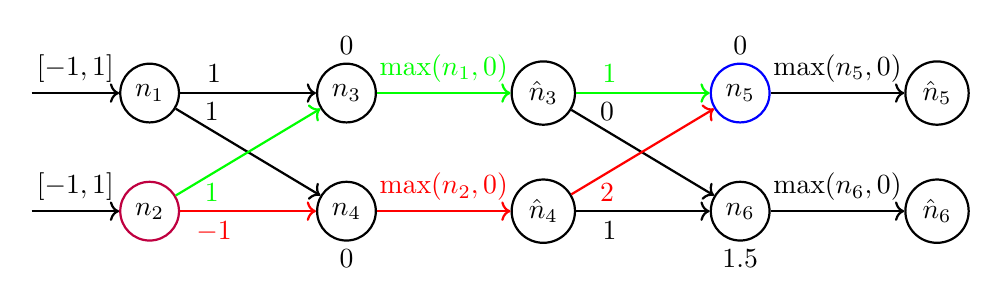
\begin{tikzpicture}
		
		\node[circle, draw= black, thick, minimum width = 20,
		minimum height = 20] (input1) {$n_1$};
		
		\node[circle, draw= purple, thick, minimum width = 20,
		minimum height = 20] (input2) at ($(input1) + (0,-1.5)$) {$n_2$};
		
		
		% Hidden layers
		
		\node (hidden10) at ($(input1) + (2.5,0.6)$) {$0$};
		
		\node (hidden20) at ($(input1) + (2.5,-1.5-0.6)$) {$0$};
		
		\node (hidden50) at ($(input1) + (7.5,0.6)$) {$0$};
		
		\node (hidden60) at ($(input1) + (7.5,-1.5-0.6)$) {$1.5$};
		
		
		\node[circle, draw= black, thick, minimum width = 20,
		minimum height = 20] (hidden1) at ($(input1) + (2.5,0)$) {$n_3$};
		\node[circle, draw= black, thick] (hidden2) at ($(input1) + (2.5,-1.5)$) {$n_4$};
		
		\node[circle, draw= black, thick, minimum width = 20,
		minimum height = 20] (hidden3) at ($(input1) + (5,0)$){$\hat{n}_3$};
		\node[circle, draw= black, thick] (hidden4) at ($(input1) + (5,-1.5)$) {$\hat{n}_4$};
		
		
		\node[circle, draw= blue, thick, minimum width = 20,
		minimum height = 20] (hidden5) at ($(input1) + (7.5,0)$){$n_5$};
		\node[circle, draw= black, thick] (hidden6) at ($(input1) + (7.5,-1.5)$) {$n_6$};
		
		
		
		
		% Output layer
		\node[circle, draw= black, thick, minimum width = 20,
		minimum height = 20] (output1) at ($(input1) + (10,0)$){$\hat{n}_5$};
		
		\node[circle, draw= black, thick, minimum width = 20,
		minimum height = 20] (output2) at ($(input1) + (10,-1.5)$){$\hat{n}_{6}$};
		
		
		% Connections
		
		\draw[->,thick] ($(input1) + (-1.5,0)$) -- (input1) node[midway, above] {$[-1,1]$};
		
		\draw[->,thick] ($(input1) + (-1.5,-1.5)$) -- (input2) node[midway, above] {$[-1,1]$};
		
		
		
		\draw[->,thick] (input1) -- (hidden1) node[near start, above] {$1$};
		\draw[->,thick] (input1) -- (hidden2)node[near start, above] {$1$};
		
		\draw[->,color=green, thick] (input2) -- (hidden1) node[near start, below] {$1$};
		\draw[->,color=red, thick] (input2) -- (hidden2)node[near start, below] {$-1$};
		
		
		
		
		
		\draw[->,color=green, thick] (hidden1) -- (hidden3) node[midway, above] {$\max(n_1,0)$};
		\draw[->,color=red, thick] (hidden2) -- (hidden4) node[midway, above] {$\max(n_2,0)$};
		
		
		
		
		
		\draw[->,color=green, thick] (hidden3) -- (hidden5) node[near start, above] {$1$};			
		\draw[->,thick] (hidden3) -- (hidden6) node[near start, above] {$0$};
		
		\draw[->,color=red, thick] (hidden4) -- (hidden5)node[near start, below] {$2$};
		\draw[->,thick] (hidden4) -- (hidden6)node[near start, below] {$1$};
		
		
		
		
		\draw[->,thick] (hidden5) -- (output1) node[midway, above] {$\max(n_5,0)$};
		\draw[->,thick] (hidden6) -- (output2) node[midway, above] {$\max(n_6,0)$};
		
		
	\end{tikzpicture}
	\caption{A DNN example from \cite{kpoly}: every neuron is separated into 2 nodes, $n$ pre- and $\hat{n}$ post-ReLU activation function. The pair $(n_2 n_3 n_5,n_2 n_4 n_5)$ in green and red is compensating (weights of paths are $1,-2$).}
	\label{fig1}
\end{figure}

The concept of value abstraction involves calculating upper and lower bounds for the values of certain neurons in a Deep Neural Network (DNN) when inputs fall within a specified range. This approach aims to assess the network's robustness without precisely computing the values for every input within that range.

Firstly, it's important to note that weighted sums represent a linear function, which can be explicitly expressed with relative ease. However, the ReLU (Rectified Linear Unit) function presents a challenge in terms of accurate representation. Although ReLU is a relatively straightforward piecewise linear function with two modes (one for $x<0$ and another for $x \geq 0$), it is not linear. The complexity arises when considering the compounded effects of the ReLU function across the various layers of a ReLU DNN. It's worth noting that representing $\ReLU(x)$ precisely is feasible when $x$ is "stable," meaning it's consistently positive or consistently negative, as there's only one linear mode involved in each scenario. Consequently, the primary challenge lies in addressing "unstable" neurons, where the linearity of the function does not hold consistently.


Consider the simpler abstraction, termed ``Box abstraction" \cite{deeppoly}: it inductively computes the bounds for each neuron in the subsequent layer independently. This is achieved by considering the weighted sum of the bounds from the previous layer, followed by clipping the lower bound at $\max(0,$ lower bound$)$ to represent the ReLU function, and so forth. For all $i$, define $x_i=\val_{\vx}(n_i)$, where $\vx=(x_1,x_2)$.

Taking the DNN example from Fig \ref{fig1}, assume $x_1,x_2 \in [-1,1]$. This implies that $x_3,x_4 \in [-2,2]$. After applying the ReLU function, $\hat{x}3,\hat{x}4$ are constrained to $[0,2]$, leading to $x_5 \in [0,6]$ and $x_6 \in [0,2]$. The bounds for $n_1, \ldots, n_4$ are exact, meaning for every $\alpha$ within the range, an input $\vy$ can be found such that $\val{\vy}(n_i)=\alpha$. However, this precision is lost from the next layer (beginning with $n_5, n_6$) due to potential dependencies among preceding neurons. For example, $n_3$ only attains the value $2$ when both $x_1$ and $x_2$ are $2$. In this case, $n_4$ would reach a value of $Val{(2,2)}(n_4)=0$. Consequently, it's implausible for $x_5=\Val_{\vx}(n_5)$ to reach $6$, as it would necessitate both $n_3$ and $n_4$ assuming the value $2$.

An extremely efficient algorithm that addresses some issues is "DeepPoly" \cite{deeppoly}, also independently discovered as the "CROWN" algorithm \cite{crown}. Instead of strict bounds, for each neuron $n$ in layer $k$, DeepPoly maintains two affine functions representing the lower and upper bounds of the neuron's value, based on inputs from the previous layer $k-1$. For instance, denote $f_i \leq x_i \leq g_i$ with, for example, $f_{3}(x_3)=f_4(x_4)=0$ and $g_3(x_3) = \frac{x_3+2}{2}$, $g_4(x_4) = \frac{x_4+2}{2}$. This leads to $x_5 \leq g_3(x_3) + 2 g_4(x_4) = \frac{x_3 + 2x_4 + 6}{2} = \frac{3x_1 - x_2 + 6}{2}\leq 5$.

For bounds $[\alpha,\beta]$ on $x_i$, the optimal linear function for the upper bound is $g_i(x_i)= \beta \frac{x_i-\alpha}{\beta-\alpha}$ for ReLU nodes. There are two options for the lower bound: $f^1_i(x_i) = 0$ or $f^2_i(x_i)=x_i$. DeepPoly selects between these based on the values of $\alpha$ and $\beta$ (for unstable neurons): if $|\alpha|\geq |\beta|$, then $f_i=f^1_i$ is chosen, otherwise, for $|\beta|>|\alpha|$, $f_i=f^2_i$ is selected. The variation, {\em $\overline{\mbox{DeepPoly}}$}, consistently chooses $f^1_i$, and never $f^2_i$. Contrary to DeepPoly, {\em $\overline{\mbox{DeepPoly}}$} encompasses the ``Box abstraction." For instance, with bounds $[-0.2,5]$ on $x_i$, it deduces $\ReLU(x_i) \in [0,5]$, whereas  DeepPoly without box abstraction algorithm would conclude $\ReLU(x_i) \in [-0.2,5]$.


\iffalse
\subsection{PRIMA and $\beta$-CROWN}
\fi

\subsection{MILP and LP encodings for DNNs}

At the other end of the spectrum, we find the Mixed Integer Linear Programming (MILP) value abstraction, which is a priori a complete method (albeit much slower than DeepPoly). 
Consider an unstable neuron $n \in[\alpha,\beta]$. The value $x$ of $\ReLU(n)$ can be encoded exactly in an MILP formula with one integer (actually even binary) variable $a$ valued in ${0,1}$, using 4 constraints \cite{MILP}:
\vspace{-0.1cm}
\begin{align*}
	\hat{x} \geq x \quad \wedge \quad \hat{x} \geq 0, \quad \wedge \quad \hat{x} \leq \beta \cdot a \quad \wedge \quad \hat{x} \leq x-\alpha \cdot (1-a)
\end{align*}

It can be shown that for all $x \in [\alpha,\beta] \setminus 0$, there exists a unique solution $(a,\hat{x})$ that meets these constraints, with $\hat{x}=\ReLU(x)$. Here, $a$ is 0 if $x < 0$, 1 if $x>0$, and can be either if $x=0$~\cite{MILP}. This encoding approach can be applied to every (unstable) ReLU node, and optimizing its value can help in certifying a given input. However, for networks with hundreds of nodes or more, the resulting MILP formulation will contain numerous integer variables and generally cannot be solved efficiently.

MILP instances can be linearly relaxed into LP over-abstraction, where variables originally restricted to integers in ${0,1}$ (binary) are relaxed to real numbers in the interval $[0,1]$, while maintaining the same encoding. As solving LP instances is polynomial time, this optimization is significantly more efficient. However, this efficiency comes at the cost of precision, often resulting in less stringent bounds. This approach is termed the {\em LP abstraction}

The following proposition shows that the LP abstraction refines the DeepPoly abstraction. 
The difference between the LP and the DeepPoly abstractions is that LP simultaneous considers the two linear lower bounding functions for the ReLU operation, namely $ReLU(x) \geq 0$ and $ReLU(x) \geq x$, while the DeepPoly abstraction restricts itself to the application of a single one of these linear bounding functions.
 

\begin{proposition}
	\label{LP}
	Given $x \in [\alpha,\beta]$ with $\alpha < 0 < \beta$, the following two systems of constraints 
	1) for LP and 2) for DeepPoly with both lower bounds are equivalent:
	\begin{align}
& \hat{x} \geq x \quad \wedge \quad \hat{x} \geq 0, \quad \wedge \quad \hat{x} \leq \beta \cdot a \quad \wedge \quad \hat{x} \leq x-\alpha \cdot (1-a), \, a \in [0,1]  \label{eq:lp}\\
&\hat{x} \geq x \quad \wedge \quad \hat{x} \geq 0 \quad \wedge \quad \hat{x} \leq \beta \frac{x-\alpha}{\beta-\alpha} \label{eq:deeppoly}
	\end{align} 
\end{proposition}

\begin{proof}
We need to show that the two upper bound constraints in Eq~\ref{eq:lp} is equivalent to the upper bound in Eq~\ref{eq:deeppoly}. To this end, we focus on the upper bound function in the linear variable $a \in  [0,1]$, with $x \in [\alpha,\beta]$ fixed. We have $\hat{x}$ in Eq~\ref{eq:lp} is upper bounded by $max_{a \in [0,1]} (min(\beta \cdot a, x - \alpha (1-a)))$, and this bound can be reached. Furthermore, 
	The function $\min(\beta \cdot a, x - \alpha (1-a))$ attains its maximum when $\beta \cdot a = x - \alpha (1-a)$, leading to the equation $(\beta - \alpha) a = x - \alpha$ and consequently $a = \frac{x - \alpha}{\beta-\alpha}$. This results in an upper bound of $\beta \cdot a = \beta \frac{x - \alpha}{\beta-\alpha}$ \qed
\end{proof}

\subsubsection*{Constraints for $\gamma$}

We could get the following constraints for $\gamma$, using $y_i$ and $\hat{y}_i$ to denote the $x_i-x_i'$ and $\hat{x}_i-\hat{x}_i'$:\begin{align*}
	\hat{y}_i \leq a \gamma_i \hspace*{2ex} &\wedge \hspace*{2ex}\hat{y} \geq y_i - a \gamma_i\\
	\hat{y}_i \geq (a-1) \gamma_i  \hspace*{2ex} &\wedge \hspace*{2ex} \hat{y} \leq y_i + (1-a) \gamma_i,
\end{align*} where $a$ is a binary variable, $\gamma_i$ is the upper bound of $x_i-x'_i$.


The following plot will show the above constraints:

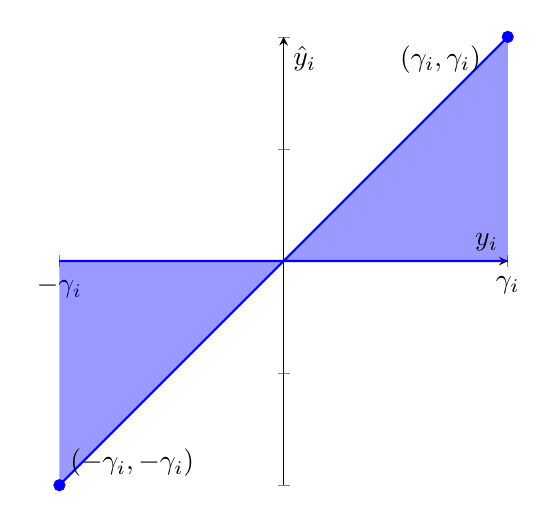
\begin{tikzpicture}
	\begin{axis}[
		xlabel={$y_i$},
		ylabel={$\hat{y}_i$},
		xmin=-2, xmax=2,
		ymin=-2, ymax=2,
		axis lines=center,
		samples=100, 
	 unit vector ratio=1 1 1, scale=1, xtick   = {-2,2},
	 xticklabels = {$-\gamma_i$,$\gamma_i$},
	 yticklabels = {},
		]
		\addplot[blue, thick, fill=blue, fill opacity=0.4] {x} \closedcycle; 
		\addplot[blue, thick] {0}; 
	
		\addplot[only marks, mark=*, mark size=2pt, blue] coordinates {(-2,-2)};
			\node[label={above:$(-\gamma_i,-\gamma_i)$}] at (axis cs: -1.35, -2.1) {};
			
				\addplot[only marks, mark=*, mark size=2pt, blue] coordinates {(2,2)};
			\node[label={above:$(\gamma_i,\gamma_i)$}] at (axis cs: 1.4, 1.5) {};
	\end{axis}
\end{tikzpicture}



The relation between $y_i$, $x'_i$ and $\hat{y}_i$ is $\hat{y}_i = \ReLU(x'_i+y_i)-\ReLU(x'_i).$ And its plots is as follows:

\hspace*{-10ex}
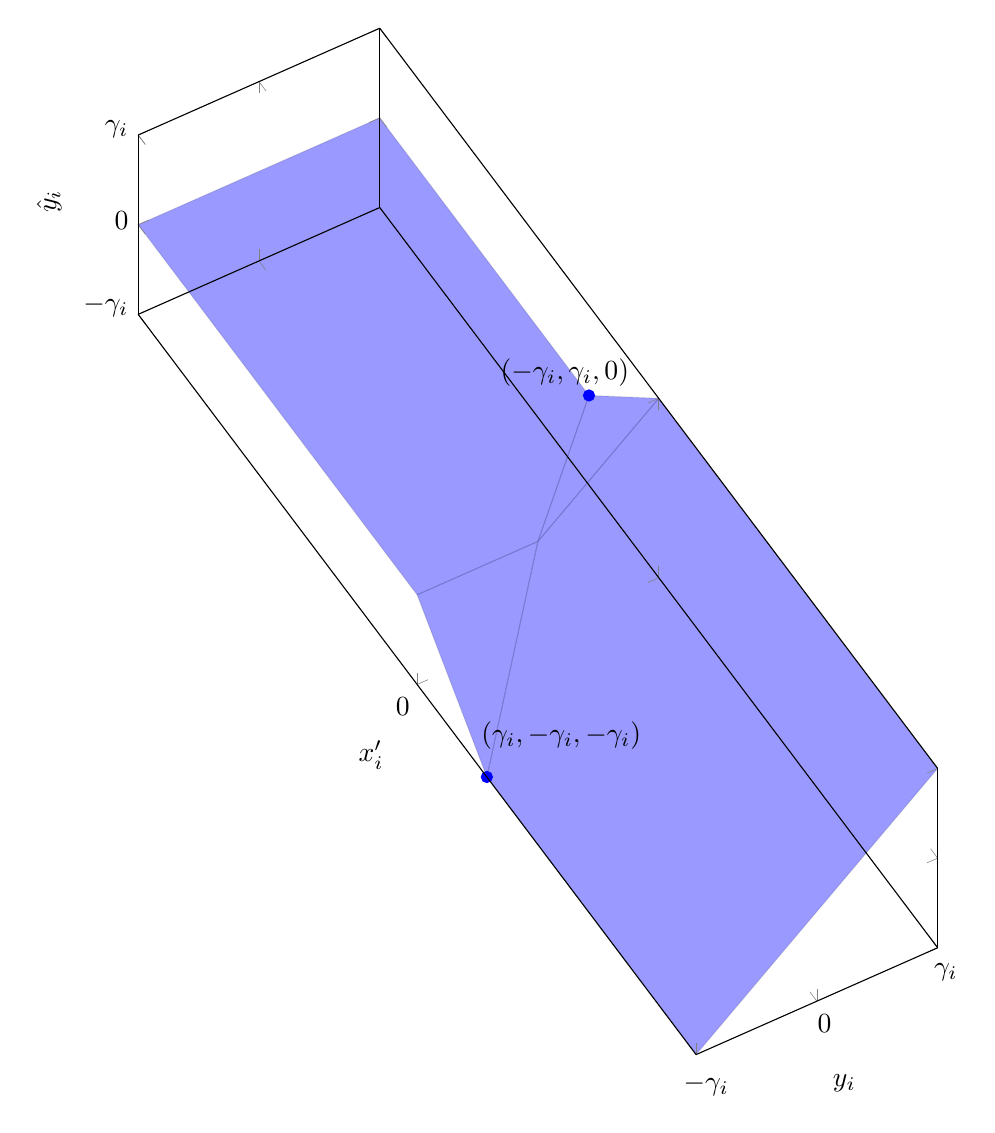
\begin{tikzpicture}
	\begin{axis}[	axis on top, xlabel = \(x'_i\),
		ylabel = {\(y_i\)}, zlabel = \(\hat{y}_i\),
				set layers=default,
	xmax = 4, xmin = -4,
ymax = 1, ymin = -1,		
zmax = 1, zmin = -1,
				unit vector ratio=1 1 1, scale=3,
				view={60}{50}, ytick   = {-1,0,1},
				yticklabels = {$-\gamma_i$,$0$,$\gamma_i$}, xtick = {0},
				xticklabels = {$0$}, ztick   = {-1,0,1},
				zticklabels = {$-\gamma_i$,$0$,$\gamma_i$},
				]
		\addplot3[fill=blue,opacity=0.1, fill opacity=0.4] 
		coordinates {
	 (0,0,0) (-1,1,0) (-4,1,0) (-4,-1,0) (0,-1,0) (0,0,0)
		};
		
		\addplot3[fill=blue,opacity=0.1, fill opacity=0.4	] 
		coordinates { (0,0,0) (0,1,1) (4, 1, 1) (4, -1, -1) (1,-1,-1) (0,0,0)
		};
		
		\addplot3[fill=blue,opacity=0.1, fill opacity=0.4	] 
		coordinates { (0,0,0)  (-1,1,0) (0,1,1) (0,0,0)
		};
		
			\addplot3[fill=blue,opacity=0.1, fill opacity=0.4	] 
		coordinates { (0,0,0)  (0,-1,0) (1,-1,-1) (0,0,0)
		};
		
		\addplot3[only marks, mark=*, mark size=2pt, blue] coordinates {(1,-1,-1)};
					\node[label={$(\gamma_i,-\gamma_i, -\gamma_i)$}] at (axis cs: 1.2, -0.5 ,-1) {};
					
			\addplot3[only marks, mark=*, mark size=2pt, blue] coordinates {(-1,1,0)};
		\node[label={$(-\gamma_i,\gamma_i, 0)$}] at (axis cs: -1, 0.8 ,0) {};			
		
	\end{axis}
\end{tikzpicture}



\hspace*{-15ex}
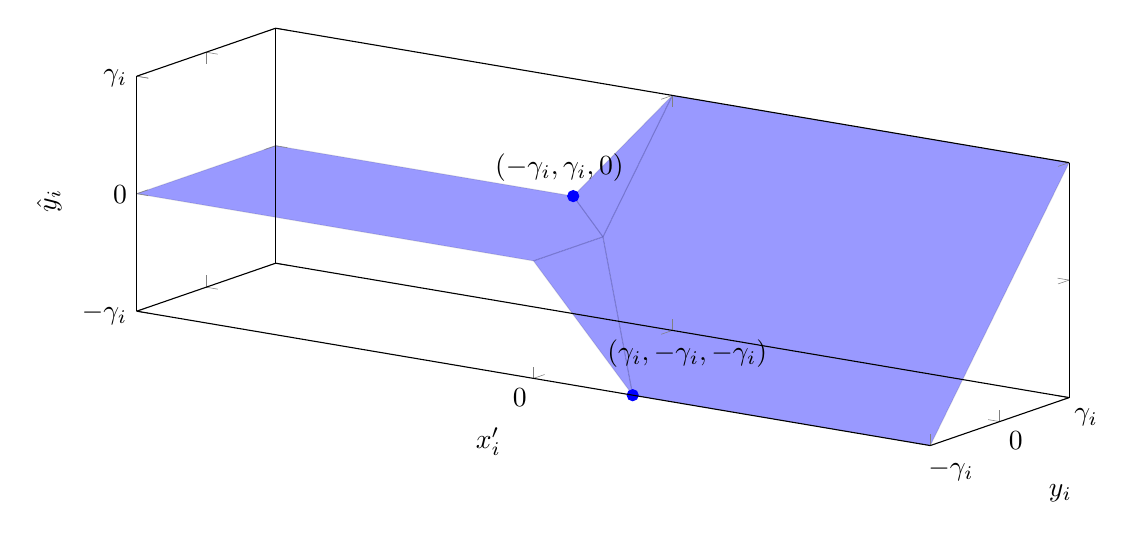
\begin{tikzpicture}
	\begin{axis}[	axis on top, xlabel = \(x'_i\),
		ylabel = {\(y_i\)}, zlabel = \(\hat{y}_i\),
		set layers=default,
				xmax = 4, xmin = -4,
		ymax = 1, ymin = -1,		
				zmax = 1, zmin = -1,
		unit vector ratio=1 1 1, scale=2.5,  ytick   = {-1,0,1},
		yticklabels = {$-\gamma_i$,$0$,$\gamma_i$}, xtick = {0},
		xticklabels = {$0$}, ztick   = {-1,0,1},
		zticklabels = {$-\gamma_i$,$0$,$\gamma_i$},
		view={35}{14},
		]
		\addplot3[ fill=blue,opacity=0.1, fill opacity=0.4] 
		coordinates {
			(0,0,0) (-1,1,0) (-4,1,0) (-4,-1,0) (0,-1,0) (0,0,0)
		};
		
		\addplot3[	fill=blue,opacity=0.1, fill opacity=0.4] 
		coordinates { (0,0,0) (0,1,1) (4, 1, 1) (4, -1, -1) (1,-1,-1) (0,0,0)
		};
		
		\addplot3[	fill=blue,opacity=0.1, fill opacity=0.4	] 
		coordinates { (0,0,0)  (-1,1,0) (0,1,1) (0,0,0)
		};
		
		\addplot3[	fill=blue,opacity=0.1, fill opacity=0.4	] 
		coordinates { (0,0,0)  (0,-1,0) (1,-1,-1) (0,0,0)
		};
		
			\addplot3[only marks, mark=*, mark size=2pt, blue] coordinates {(1,-1,-1)};
		\node[label={$(\gamma_i,-\gamma_i, -\gamma_i)$}] at (axis cs: 1.2, -0.5 ,-1) {};
		
		\addplot3[only marks, mark=*, mark size=2pt, blue] coordinates {(-1,1,0)};
		\node[label={$(-\gamma_i,\gamma_i, 0)$}] at (axis cs: -1, 0.8 ,0) {};			
		
	\end{axis}
\end{tikzpicture}


%\begin{tikzpicture}[
%	declare function={
%		f(\x,\y)=max((\x+\y),0)-max(\x,0);
%	}]
%	\begin{axis}[axis lines=center,
%		axis on top,
%		set layers=default,
%		xrange=-3:3,
%		yrange=-2:2,
%		unit vector ratio=1 1 1,% <- HERE (taken from Phelype Oleinik's deleted answer)
%		scale=3 %<- added to compensate for the downscaling
%		% resulting from unit vector ratio=1 1 1
%		]
%		\addplot3[
%		domain=-3:3,
%		domain y=-1:1, surf,
%		samples=40,
%		samples y=40,
%		] {f(\x,\y)};
%	\end{axis}
%\end{tikzpicture}
 


\section{Global Scoring Functions}

\label{sec4p5}

First, we adapt from the BaB-SR \cite{BaB} and FSB \cite{FSB} functions (replacing the symbols from the original paper with those used in our paper.), selecting a node to branch on for BaB, {\em  global scoring} (GS) functions to select nodes for pMILP. Intuitively, we extract the scoring $s_{SR}$ and $s_{FSB}$ from both BaB-SR and FSB, as the BaB bounding step is not adapted for pMILP. They both work by backpropagating gradients vectors $\bm{\lambda}$ from the neurons under consideration in layer $n$, back to neurons to be potentially selected. To do so, they consider the rate of $\ReLU(\bm{u}_k)$ to be 
$r(\bm{u}_k)=\frac{\max(0,\UB(\bm{u}_k))}{\max(0,\UB(\bm{u}_k))-\min(0,\LB(\bm{u}_k))} \in [0,1]$, 
with $r(b)=0$ iff $\UB(b)\leq 0$ and $r(b)=1$ iff $\LB(b)\geq 0$.

\begin{align*}
\bm{\lambda}_{n-1} = -{(\bm{W}^n)}^T\bm{1}, \hspace*{4ex}  	\bm{\lambda}_{k-1} = {(\bm{W}^k)}^T\big( r(\bm{u}_k) \odot\bm{\lambda}_{k}\big) \hspace*{4ex}  k\in [n-1,2]
\end{align*}


Then, the scoring functions $\bm{s}_{SR}$ and $\bm{s}_{FSB}$ for ReLUs in layer $k$ are computed by approximating how each node would impact the neurons in layer $n$, by also factoring in the bias $\bm{b}_k$ in different ways:

\begin{align*}
	\bm{s}_{SR}(k) =& %\bm{1}_{\bm{u}_k>0,\bm{l}_k<0} \odot
	\Biggl\lvert r(\bm{u}_k) \odot \LB(\bm{u}_k) \odot \max(\bm{\lambda}_{k},0)
	+ \max\{0,\bm{\lambda}_{k}\odot\bm{b}_{k}\}-r(\bm{u}_k) \odot\bm{\lambda}_{k}\odot\bm{{b}}_{k}
	\Biggr\rvert  \\
	\bm{s}_{FSB}(k) =& \Biggl\lvert r(\bm{u}_k) \odot \LB(\bm{u}_k) \odot \max(\bm{\lambda}_{k},0)
	+ \min\{0,\bm{\lambda}_{k}\odot\bm{b}_{k}\}-r(\bm{u}_k) \odot\bm{\lambda}_{k}\odot\bm{{b}}_{k}
	\Biggr\rvert
\end{align*}

In case where the bias is 0, then there is no difference between $s_{SR}$ and $s_{FSB}$.
Then, unstable ReLU (with $\LB(u_k) < 0 < \UB(u_k)$) are ranked using these scores, to select the most important ReLUs, as stable ReLUs are linear, thus they are already treated correctly.


\begin{figure}[t!]
	\centering
	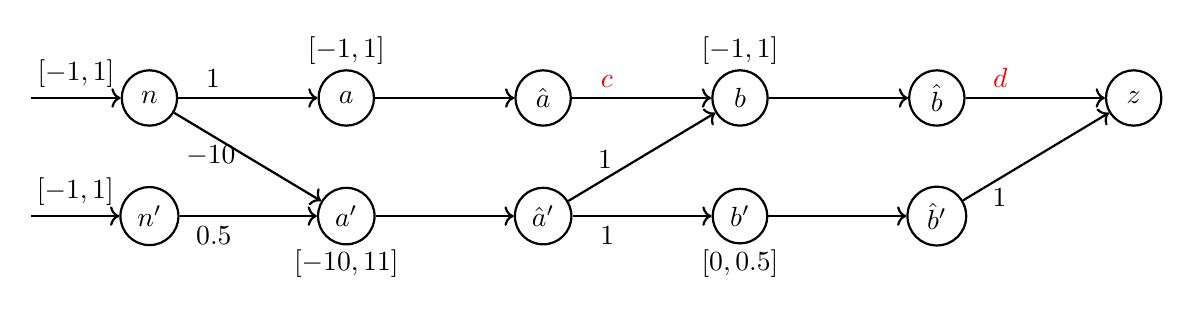
\begin{tikzpicture}
		
		\node[circle, draw= black, thick, minimum width = 20,
		minimum height = 20] (input1) {$n$};
		
		\node[circle, draw= black, thick, minimum width = 20,
		minimum height = 20] (input2) at ($(input1) + (0,-1.5)$) {$n'$};
		
		
		% Hidden layers
		
		\node (hidden10) at ($(input1) + (2.5,0.6)$) {$[-1,1]$};
		
		\node (hidden20) at ($(input1) + (2.5,-1.5-0.6)$) {$[-10,11]$};
		
		\node (hidden50) at ($(input1) + (7.5,0.6)$) {$[-1,1]$};
		
		\node (hidden60) at ($(input1) + (7.5,-1.5-0.6)$) {$[0,0.5]$};
		
		
		\node[circle, draw= black, thick, minimum width = 20,
		minimum height = 20] (hidden1) at ($(input1) + (2.5,0)$) {$a$};
		\node[circle, draw= black, thick] (hidden2) at ($(input1) + (2.5,-1.5)$) {$a'$};
		
		\node[circle, draw= black, thick, minimum width = 20,
		minimum height = 20] (hidden3) at ($(input1) + (5,0)$){$\hat{a}$};
		\node[circle, draw= black, thick] (hidden4) at ($(input1) + (5,-1.5)$) {$\hat{a}'$};
		
		
		\node[circle, draw= black, thick, minimum width = 20,
		minimum height = 20] (hidden5) at ($(input1) + (7.5,0)$){$b$};
		\node[circle, draw= black, thick] (hidden6) at ($(input1) + (7.5,-1.5)$) {$b'$};
		
		
		
		
		% Output layer
		\node[circle, draw= black, thick, minimum width = 20,
		minimum height = 20] (output1) at ($(input1) + (10,0)$){$\hat{b}$};
		
		\node[circle, draw= black, thick, minimum width = 20,
		minimum height = 20] (output2) at ($(input1) + (10,-1.5)$){$\hat{b}'$};
		
			\node[circle, draw= black, thick, minimum width = 20,
		minimum height = 20] (output3) at ($(input1) + (12.5,0)$){$z$};
		
		
		% Connections
		
		\draw[->,thick] ($(input1) + (-1.5,0)$) -- (input1) node[midway, above] {$[-1,1]$};
		
		\draw[->,thick] ($(input1) + (-1.5,-1.5)$) -- (input2) node[midway, above] {$[-1,1]$};
		
		\draw[->,thick] (input1) -- (hidden1) node[near start, above] {$1$};
		\draw[->,thick] (input1) -- (hidden2)node[near start, below] {$-10$};
		
		\draw[->, thick] (input2) -- (hidden2)node[near start, below] {$0.5$};
		
		
		
		
		
		\draw[->, thick] (hidden1) -- (hidden3);
		\draw[->, thick] (hidden2) -- (hidden4);
		
		
		
		
		
		\draw[->, thick] (hidden3) -- (hidden5) node[near start, above] {{\color{red}$c$}};			
	
		\draw[->,thick] (hidden4) -- (hidden5)node[near start, above] {$1$};
		\draw[->,thick] (hidden4) -- (hidden6)node[near start, below] {$1$};
		
		
		\draw[->,thick] (hidden5) -- (output1);
		\draw[->,thick] (hidden6) -- (output2);
		
		\draw[->,thick] (output1) -- (output3)node[near start, above] {{\color{red}$d$}};
		\draw[->,thick] (output2) -- (output3)node[near start, below] {$1$};
		
		
	\end{tikzpicture}
	\caption{A simple example with parametric weights {\color{red}$c$} and {\color{red}$d$}}
	\label{img:FSB_example}
\end{figure}




Consider the example in Fig. \ref{img:FSB_example}. It has no bias so $s_{SR}=s_{FSB}$.
We have $\lambda(b)=d$, $\lambda(a)=\frac{cd}{2}$.
Let us do a case analysis:
The most favorable cases are $c < 0 < d$ and $d < 0 < c$: 
as $cd <0$, we have $s_{FSB}(a)=\max(0,\frac{cd}{4}) = 0$.
Now, $a$ and $\hat{a}$ need to be minimized in order to maximize $z$, because $cd <0$. 
For the triangle approximation (see Fig. \ref{triangle}), having a value $sol(a)$ for $a$, the minimal value for $\hat{a}$ is $\ReLU(sol(a))$. If we open $a$, then the value for $\hat{a}$ will also be $\ReLU(sol(a))$. That is, opening this ReLU is not helping in the approximation of $z$, as correctly predicted by the score $s_{FSB}(a)= 0$.



Case $c>0,d>0$: $s_{FSB}(a)=\frac{cd}{4}$.
The value of $a,\hat{a},b,\hat{b}$ should be maximized to maximize the value of $z$, because $W_{bz}=d>0$ and $W_{ab}=c>0$. 
%Each variation of $b$ by $\Delta(b)$ will have an impact $r(b) \cdot \Delta(b)=\frac{\Delta(b)}{2}$ on the value of $\hat{b}$, and thus $\frac{d \Delta(b)}{2}$ on $z$. 
Now, let us call $sol(a)$ the maximum value for $a$.
The maximum value for $\hat{a}$ is $r(a)\cdot (sol(a)-LB(a))$ according to the triangle approximation when $\ReLU(a)$ is not opened. Now, if $\ReLU(a)$ is opened, then 
the value of $\hat{a}$ is $\ReLU(sol(a))$: the difference is at most $r(a) \cdot LB(a) = \frac{1}{2}$. The difference $\Delta(b)$ for the value of $b$ is thus at most $\frac{c}{2}$, which means a difference at most $\frac{c}{4}$ for $\hat{b}$, using the upper function of the triangle approximation of rate $r(b)$, as the value of $\hat{b}$ should be maximized.
This means a difference of at most $\frac{cd}{4}$ on the value of $z$, which is what is computed by $s_{FSB}(a)$. Of course, the difference of opening $\ReLU(a)$ could also be 0 e.g. if $\sol(a)=\LB(a)$ or $\sol(a)=\UB(a)$.

The last case is the most problematic: 
Case $c<0,d<0$, implying that $s_{FSB}(a)=\frac{cd}{4}$, because $cd >0$.
As for the case of $c>0, d>0$, opening $\ReLU(a)$ will have an impact on the value of $\hat{a}$,
at most $\frac{1}{2}$, and hence a change $\Delta(b)$ of at most $\frac{c}{2}$ on the value of $b$.
However, as $d<0$, value of $\hat{b}$ needs to be minimized. That is, the value of $\hat{b}$ will be the value of $\ReLU(sol(b))$, and the change in $\hat{b}$ will be either 0 in case $sol(b)<0$ (phase 0 of ReLU),
or $\Delta(b)<\frac{c}{2}$ otherwise (phase Id of ReLU), that is, $z$ will be modified by 
either 0 or $d \Delta(b)<\frac{cd}{2}$, as compared with $s_{FSB}(a)=\frac{cd}{4}$.



\begin{figure}[t!]
	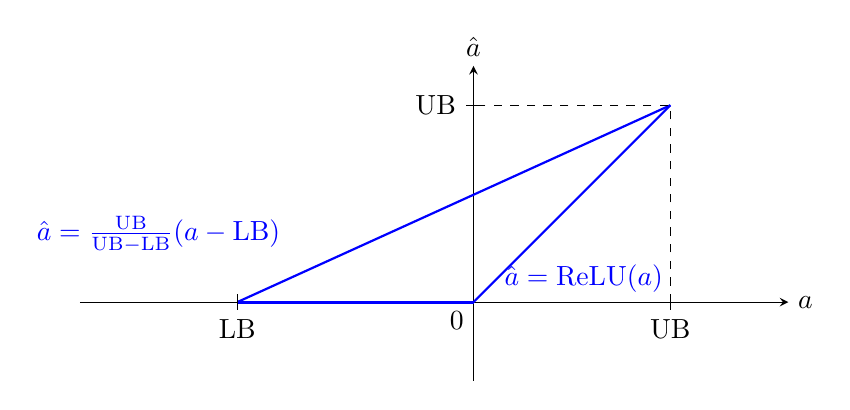
\begin{tikzpicture}[scale=1, >=stealth]
		
		% Draw axes
		\draw[->] (-5,0) -- (4,0) node[right] {$a$};
		\draw[->] (0,-1) -- (0,3) node[above] {$\hat{a}$};
		
		% Draw ReLU function
		\draw[line width=0.4mm, blue] (-3,0) -- (0,0);
		\draw[thick, blue] (0,0) -- (2.5,2.5) node[below, shift={(-1.1,-1.9)}] {$\hat{a} = \ReLU(a)$};
		\draw[thick, blue] (-3,0) -- (2.5,2.5) node[above, shift={(-6.5,-2)}] {$\hat{a} = \frac{\UB}{\UB-\LB} (a-\LB)$};
		
		% Add labels
		\draw[dashed] (2.5,0) -- (2.5,2.5) -- (0,2.5); % Optional grid
		\node[below left] at (0,0) {$0$};
		
		% Add tick marks
		
		\foreach \x in {2.5}
		\draw[shift={(\x,0)}] (0,0.1) -- (0,-0.1) node[below] {$\UB$};
		\foreach \x in {-3}
		\draw[shift={(\x,0)}] (0,0.1) -- (0,-0.1) node[below] {$\LB$};
	
		\foreach \y in {2.5}
		\draw[shift={(0,\y)}] (0.1,0) -- (-0.1,0) node[left] {$\UB$};
		
		
	\end{tikzpicture}
		\caption{Triangle approximation}
	\label{triangle}
	\end{figure}



\begin{figure}[t!]
	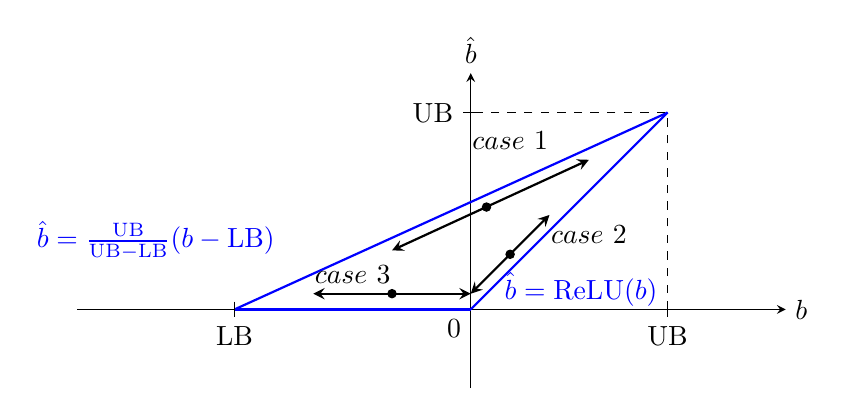
\begin{tikzpicture}[scale=1, >=stealth]
		
		% Draw axes
		\draw[->] (-5,0) -- (4,0) node[right] {$b$};
		\draw[->] (0,-1) -- (0,3) node[above] {$\hat{b}$};
		
		% Draw ReLU function
		\draw[line width=0.4mm, blue] (-3,0) -- (0,0);
		\draw[thick, blue] (0,0) -- (2.5,2.5) node[below, shift={(-1.1,-1.9)}] {$\hat{b} = \ReLU(b)$};
		\draw[thick, blue] (-3,0) -- (2.5,2.5) node[above, shift={(-6.5,-2)}] {$\hat{b} = \frac{\UB}{\UB-\LB} (b-\LB)$};
		
		% Add labels
		\draw[dashed] (2.5,0) -- (2.5,2.5) -- (0,2.5); % Optional grid
		\node[below left] at (0,0) {$0$};
		
		% Add tick marks
		
		\foreach \x in {2.5}
		\draw[shift={(\x,0)}] (0,0.1) -- (0,-0.1) node[below] {$\UB$};
		\foreach \x in {-3}
		\draw[shift={(\x,0)}] (0,0.1) -- (0,-0.1) node[below] {$\LB$};
		
		\foreach \y in {2.5}
		\draw[shift={(0,\y)}] (0.1,0) -- (-0.1,0) node[left] {$\UB$};
		
		\draw[<->, thick] (0, 0.2) -- (1, 1.2) node[above,shift={(0.5,-0.5)}] {$case\ 2$};
		\filldraw[black] (0.5, 0.7) circle (1.5pt);
		
		\draw[<->, thick] (0, 0.2) -- (-2, 0.2) node[above,shift={(0.5,0)}] {$case\ 3$};
		\filldraw[black] (-1, 0.2) circle (1.5pt);
		
		
		\draw[<->, thick] (-1, 0.75) -- (1.5, 1.9) node[above,shift={(-1,0)}] {$case\ 1$};
		\filldraw[black] (0.2, 1.3) circle (1.5pt);
		
	\end{tikzpicture}
	\caption{Different cases of node $b$}
	\label{node:b}
\end{figure}

We call {\em global scoring} (GS) such functions $s_{FSB},s_{SR}$  because they score ReLUs as accuratly as possible, considering that they do not have access to the solution $sol(a),sol(b)$ values. This analysis already hints at our novel ranking function, that will be solution-aware to be more accurate.
	



\iffalse
\begin{figure}[t!]
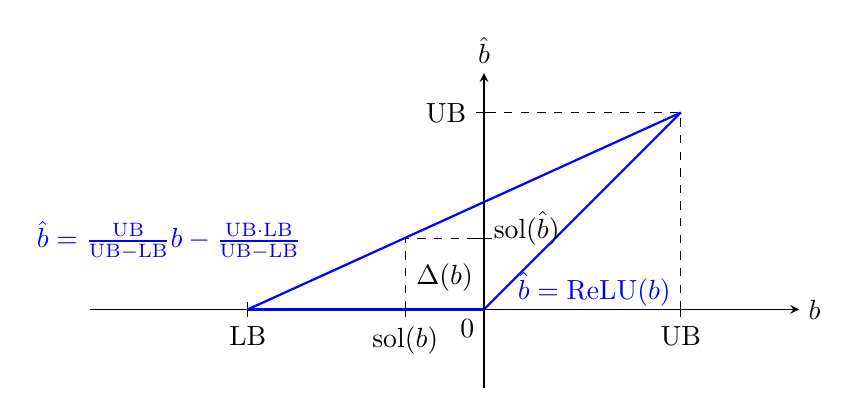
\begin{tikzpicture}[scale=1, >=stealth]
	
	% Draw axes
	\draw[->] (-5,0) -- (4,0) node[right] {$b$};
	\draw[->] (0,-1) -- (0,3) node[above] {$\hat{b}$};
	
	% Draw ReLU function
	\draw[line width=0.4mm, blue] (-3,0) -- (0,0);
	\draw[thick, blue] (0,0) -- (2.5,2.5) node[below, shift={(-1.1,-1.9)}] {$\hat{b} = \ReLU(b)$};
	\draw[thick, blue] (-3,0) -- (2.5,2.5) node[above, shift={(-6.5,-2)}] {$\hat{b} = \frac{\UB}{\UB-\LB} b-\frac{\UB\cdot\LB}{\UB-\LB}$};
	
	% Add labels
	\draw[dashed] (2.5,0) -- (2.5,2.5) -- (0,2.5); % Optional grid
	\node[below left] at (0,0) {$0$};
	
	% Add tick marks
	
	\foreach \x in {2.5}
	\draw[shift={(\x,0)}] (0,0.1) -- (0,-0.1) node[below] {$\UB$};
	\foreach \x in {-3}
	\draw[shift={(\x,0)}] (0,0.1) -- (0,-0.1) node[below] {$\LB$};

	\foreach \y in {2.5}
	\draw[shift={(0,\y)}] (0.1,0) -- (-0.1,0) node[left] {$\UB$};
	
	\draw (-1,0.1) -- (-1,-0.1) node[below] {$\sol(b)$};
	\draw[dashed] (-1,0) -- (-1,0.9) -- (0,0.9);
	\draw (-0.1,0.9) -- (0.1,0.9) node[right, shift={(-0.1,0.13)}] {$\sol(\hat{b})$};
	\node at (-0.5,0.4) {$\Delta(b)$};
	
\end{tikzpicture}
	\caption{}
\label{img:Utility}
\end{figure}
\fi


\iffalse
\subsection*{An example when FSB is not accurate}

See the figure \ref{img:FSB_example}. When the algorithm considers neurons in the layer of $a,a'$, FSB will think $a$ is important, but Utility will think it is not important (Utility value is 0).

Although this example is extreme, similar situations frequently occur in practice.

\subsection*{Comparison on MNIST}

Here we use the network named MNIST $5\times 100$ and a hard image to compare the effect of FSB and Utility function. 

We fix an intermediate bound data for layers before the third hidden layer, and use different methods based on this bound to compute the upper and lower bounds of neurons in the second and third hidden layer.

The plot shows that when only considering neurons in one layer before the target layer, we are significantly better.


\subsection*{Comparison on CIFAR10}

Here we use the network named CNN-B-adv and a hard image to compare the effect of FSB and Utility function. 

We fix an intermediate bound data for layers before the target layers, and use different methods based on this bound to compute the output layer.

The plot shows that our Utility function is significantly better than FSB, and other methods.
\fi



\section{Solution-Aware Scoring.}

\label{sec4}

In this section, we propose a novel {\em Solution-Aware Scoring} (SAS),
to evaluate accurately how opening a ReLU impacts the accuracy.
To do so, SAS considers explicitly the {\em difference} $\Delta(z)$ on the value of target node $z$ from opening $\ReLU(a)$, that is the difference for the value of $z$ between considering $\ReLU(a)$ exactly or using its LP relaxation $\LP(a)$, using the solution to a unique full LP call, which is resonnably fast to obtain. To compute $\Delta(z)$, intermediate $\Delta(b),\Delta(\hat{b})$ are computed inductively.
%Indeed, it is not rare that $z$ is sensitive to ReLU node $n$, and yet $\LP(n)$ already provides an accurate approximation of $\ReLU(n)$.
%In this case, usual heuristics would open $n$, while it would only improve the value of $z$ in a limited way.

Assume that we want to compute an upper bound for neuron $z$ on layer $\ell_z$.
We write $n < z$ if neuron {\color{blue} $n$ is} on a layer before $\ell_z$, and $n \leq z$ if $n< z$ or $n=z$. We denote ($\Sol\_\max_X^z(n))_{n \leq z}$ a solution of $\mathcal{M}_X$ maximizing $z$. In particular, $\Sol\_\max_X^z(z)$ is the maximum of $z$ under $\mathcal{M}_X$.

Consider $(sol(n))_{n \leq z} = (\Sol\_\max_\emptyset^z(n))_{n \leq z}$, a solution maximizing the value for $z$ when all ReLU use the LP relaxation.
%(this can be obtained very efficiently by {\em one} call to an LP solver).
Function
$\Improve\_\max^z(n)=$ $\sol(z) - \Sol\_\max_{\{n\}}^z(z)$, 
accurately represents how much opening neuron $n < z$ reduces the maximum computed for $z$
compared with using only LP. 
We have $\Improve\_\max^z(n)\geq 0$ as $\Sol\_\max_{\{n\}}^z$ fulfills all the constraints of 
$\mathcal{M}_\emptyset$, so $\Sol\_\max_{\{n\}}^z(z) \leq \sol(z)$.
Similarly, we define ($\Sol\_\min_\emptyset^z(n))_{n \leq z}$ and 
$\Improve\_\min^z(n)$. Calling MILP on $\mathcal{M}_{\{n\}}$ for every neuron $n \leq z$
would however be very time consuming when the number of neurons $a$ to evaluate is large.
{\color{blue} 
The main novelty of our SAS function is that it uses a (single) LP call to compute $(sol(n))_{n \leq z}$, with negligible runtime wrt the forthcoming  $\MILP_X$ call, and yet accurately approximates $\Improve\_\max^z(n)$ to choose a meaningful set $X$ of open nodes (Table \ref{tab:example1}).


\iffalse
That's why as far as we know, in competing heuristics to rank important nodes (e.g. \cite{BaB,huang2017safety,ferrari2022complete}), no call to solvers are made.
%Instead, we focus on the following $\Utility\_\max\nolimits^z(n)$ function upper bounding $\Improve\_\max^z(n)$. 
\fi





%\subsubsection*{Observation}

%The key of our formula is based on the following observation:



%Our observation (by experiments) is that \begin{align}
%	I_X \approx \sum_{b\in X} I_b.
%\end{align} Especially, if all neurons in $X$ are from one layer before $a$, then in %experiments, we observe that 

\iffalse
\begin{align*}
	|(I_X - \sum_{b\in X} I_b)/I_X| < 1\%. \ (\text{in experiments})
\end{align*} Even $X$ contains neurons from 3 layers before the target layer, in experiments, $I_X$ is still close to $\sum_{b\in X} I_b$.

Therefore, based on this observation, the question to choose $X$ is converted to compute $I_b$ for neurons $b$ in layers before the target layer. Our formula is to estimate the improvement of different individual neurons in different layers. For different layers, the formula will be different.  However, neither the observation in this subsection nor the formula in the next subsection has solid theoretical proof to show that they are very accurate. They are all based on experiments. 


In our algorithm, we will open neurons at most 3 layer3 before the target layer. So the formula will consists of three parts.


\subsubsection*{Compute the improvement of a single neuron}

\subsection*{One Layer before $z$}

\fi

%For all neurons $n$, let $\sol(n)=$$\Sol\_\max_\emptyset^z(n)$ be the value of neuron $a$
%in the solution of the LP instance $\Sol\_\max_\emptyset^z$ to maximize $z$.
%For one layer before the target layer, the formula is simple and most accurate. 
%To estimate $\Improve\_\max^z(a)$, 



%we define $\Utility\_\max^z(a)$, first for neurons $a$ one layer before $z$, by computing by how much the value of $z$ will change if $a$ is opened
%and other values remain the same - in particular, $value(\hat{a})=\ReLU(sol(a))$. We define:
%we first need to run $M^a_{\emptyset}$ to compute the upper bound of $a$  to obtain the solution data. Especially, we will read the values of $b$, before $\ReLU$ function and after $\ReLU$ function.

For a neuron $b$ on the layer before the layer $\ell_z$, we define:


\vspace{-0.4cm}
	$$\Utility\_\max\nolimits^z(b) = W_{bz} \times (\sol(\hat{b})- \ReLU(\sol(b)))$$
\vspace{-0.4cm}
	
	%In particular, if $\sol(\hat{a})=\ReLU(\sol(a))$, then we will have 
	%\begin{align*}
%		Utility^z(a) = 0.
%	\end{align*}

Consider $b$ with $W_{bz}<0$: to maximize $z$, the value of $\sol(\hat{b})$ is minimized, 
which is $\sol(\hat{b})=\ReLU(\sol(b))$ thanks to Proposition~\ref{LP}. 
Even if $z$ is sensitive to this ReLU $b$, the improvement of $b$ is 0.
Utility does not open it as $\Utility\_\max^z(b)=0$, whereas usual heuristics would.

Recall the rate $r(b)=\frac{\max(0,\UB(b))}{\max(0,\UB(b))-\min(0,\LB(b))} \in [0,1]$.
For a neuron $a$ two layers before $\ell_z$, 
$b$ denoting neurons in the layer $\ell$ just before $\ell_z$, 
we define:

\begin{align*}
	\Delta(\hat{a}) &= \ReLU(\sol(a))-\sol(\hat{a})\\
	\forall b \in \ell, \Delta(b) &= W_{ab}\Delta(\hat{a})\\
	\forall b \in \ell, \Delta(\hat{b}) &=
	\begin{cases}
		%\Delta(b),  & \text{if } W_{bz} > 0 \text{ and } \LB(b)\geq 0\\
		r(b)\Delta(b),%\frac{\UB(b)}{\UB(b)-\LB(b)}\Delta(b),  
		&\text{if }W_{bz} > 0 \\ % \text{ and } \LB(b)<0\\
		\max(\Delta(b),-\sol(b)),  &\text{if }  W_{bz} < 0 \text{ and } \sol(b)\geq0\\
		\max(\Delta(b)+\sol(b),0),  &\text{if }  W_{bz} < 0 \text{ and } \sol(b)<0		 
	\end{cases}\\
	\Utility\_\max\nolimits^z(a) &= -\sum_{b \in \ell} W_{bz} \Delta(\hat{b})
\end{align*}

%\begin{tikzpicture}[scale=1, >=stealth]
%	
%	% Draw axes
%	\draw[->] (-5,0) -- (4,0) node[right] {$x$};
%	\draw[->] (0,-1) -- (0,3) node[above] {$y$};
%	
%	% Draw ReLU function
%	\draw[line width=0.4mm, blue] (-3,0) -- (0,0);
%	\draw[thick, blue] (0,0) -- (2.5,2.5) node[below, shift={(0.5,-0.4)}] {$y = \ReLU(x)$};
%	\draw[thick, blue] (-3,0) -- (2.5,2.5) node[above, shift={(-0.5,0.4)}] {$y = \frac{\UB}{\UB-\LB} x-\frac{\UB\LB}{\UB-\LB}$};
%	
%%	% Add labels
%%	\draw[dashed] (2,0) -- (2,2) -- (0,2); % Optional grid
%%	\node[below left] at (0,0) {$0$};
%%	
%%	% Add tick marks
%%	\foreach \x in {1,2}
%%	\draw[shift={(\x,0)}] (0,0.1) -- (0,-0.1) node[below] {\x};
%%	\foreach \y in {1,2}
%%	\draw[shift={(0,\y)}] (0.1,0) -- (-0.1,0) node[left] {\y};
%	
%\end{tikzpicture}

%We will show with a more general definition that $0 \leq \Improve\_\max^z(a) \leq \Utility\_\max^z(a)$ in Prop.~\ref{prop2}. 

%Informally, $\Delta(\hat{a}), \Delta(b), \Delta(\hat{b})$ approximate the improvement on the accuracy of $\hat{a}, b, \hat{b}$ when computing $\ReLU(a)$ using the exact MILP encoding instead of LP. 

Notice that $\Utility$ does not need to consider bias explicitly, unlike $s_{FSB},s_{SR}$,
as they are already accounted for in the solution considered. 
There are two main differences with $s_{FSB}$: 
First, $\Delta(\hat{a})$ is defined exactly, with $\ReLU(\sol(a))-\sol(\hat{a})$,
whereas the corresponding $\Delta_{FSB}(\hat{a})$ is approximated as $\LB(a) r(a)$, 
which is only an upper bound of $\ReLU(\sol(a))-\sol(\hat{a})$.
More importantly, the corresponding $\Delta_{FSB}(\hat{b})$ is always $r(b) \Delta(b)$, whereas SAS adapts to the case when $W_{bz}<0$, correctly considering the 0 phase of $ReLU(b)$ when $\sol(b)\geq 0$, and the ID phase when $\sol(b)<0$.
Assuming that the solution to maximize $z$ does not change when opening $\ReLU(a)$
on neurons independant of $a$, then $\Utility$ is exact. This is not the case for $s_{FSB}$ because of the two previously mentionned cases. Further, even when the global solution changes, we can show that $\Utility$ is a safe overapproximation, which does not hold for $s_{FSB},s_{SR}$ (because of the case $sol(b) > 0$):
}

\begin{proposition}
	\label{prop2}
		$0 \leq \Improve\_\max^z(a) \leq \Utility\_\max^z(a)$. 
\end{proposition}


Thus, $\Utility\_\max^z(a)$ can be used to approximate $\Improve\_\max^z(a)$. 
In particular, for all nodes $a$ with $\Utility\_\max\nolimits^z(a)=0$, 
we are sure that this node is not having any impact on $\Sol\_\max_{\{a\}}^z(z)$. 
%This is one striking difference (but not the only one) with choosing utility based on 
%$|W_{az}|$ \cite{DivideAndSlide}.

	
%	
%	Similarly, let $\sol(b)$ be the value of $b$ in the LP solution of lower bound of $a$, and $\sol(\hat{b})$ be the value of $\hat{b}$. Then the formula to estimate improvement of lower bound of $b$ is: \begin{align*}
%		Improve\_min^z(b) \approx -W_{ba}(\sol(\hat{b})-\ReLU(\sol(b))).
%	\end{align*}
	
%To explain the formula, we use upper bound and the case that $W_{ba} > 0$ as an example. To compute the upper bound of $a$, $\hat{b}$ should be as large as possible. In the LP model, for fixed $\sol(b)$, the upper bound of $\hat{b}$ may be larger than $\ReLU(\sol(b))$. This is because in LP model, the upper bound of $\sol(\hat{b})$ is decided by the linear approximation rather than $\ReLU$ function. So, when neuron $b$ is open, if $\sol(b)$ do not change, then the upper bound of $a$ will be improved because the value of $\sol(\hat{b})$ will be lower to $\ReLU(\sol(b))$.
% 			
%Of course changing other variables may also effect the upper bound, but our experiments show that, the change from $\sol(\hat{b})$ to $\ReLU(\sol(b))$ is the major part of improvement. 


 



	
	\begin{proof}
    Consider $\sol'(n)_{n \leq z}$ with
	$\sol'(n)=\sol(n)$ for all $n \notin \{z,\hat{a}\} \cup \{b,\hat{b} \mid b \in \ell\}$. In particular,  $\sol'(a) = \sol(a)$.
	Now, define $\sol'(\hat{a}) = \ReLU(\sol(a))$. 
	That is, $\sol'(\hat{a})$ is the correct value for $\hat{a}$, obtained if we open neuron $a$, compared to the LP abstraction for $\sol(\hat{a})$.
	We define $\sol'(b)=\sol(b)+\Delta(b)$ and 
	$\sol'(\hat{b})=\sol(\hat{b}) + \Delta(\hat{b})$.
	Last, $\sol'(z)=\sol(z) + \sum_{b \in \ell} W_{bz} \Delta(\hat{b})$.
	We will show:
	\begin{equation}
		\label{eq12}
		(\sol'(n))_{n \leq z} \text{ satisfies the constraints in } \mathcal{M}_{\{a\}}
	\end{equation} 
	This suffices to conclude: as
	$\sol'(z)$ is a solution of $\mathcal{M}_{\{a\}}$, it is smaller or equal to the maximal solution: $\sol'(z) \leq$ $\Sol\_\max_{\{a\}}^z(z)$. That is, 
	$\sol(z)-\sol'(z) \geq \sol(z) -$ $\Sol\_\max_{\{a\}}^z(z)$, i.e. 
	$ \Utility\_\max^z(a) \geq \Improve\_\max^z(a)$.
	In particular, we have that $\Utility\_\max^z(a) \geq 0$, which was not obvious from the definition.

	Finally, we show (\ref{eq12}). First, opening $a$ changes the value of $\hat{a}$ from
	$\sol(\hat{a})$ to $\ReLU(\sol(a)) = sol(\hat{a}) + \Delta(a)$, 
	and from $sol(b)$ to $sol(b) + \Delta(b)$.
	The case of $\Delta(\hat{b})$ is the most interesting:
	If $W_{bz}>0$, then according to Proposition \ref{LP}, the LP solver
sets $\sol(\hat{b}) = \sol(b) \frac{\UB(b)}{\UB(b)-\LB(b)} +$ Cst to maximize $z$.
Changing $b$ by $\Delta(b)$ thus results in changing $\sol(\hat{b})$ by 
$\frac{\UB(b)}{\UB(b)-\LB(b)}\Delta(b)$.
If $W_{bz}\leq0$, then the LP solver sets $\sol(\hat{b})$ to the lowest possible value to maximize $z$, which happens to be $\ReLU(b)$ according to Proposition \ref{LP}.
If $\sol(b) < 0$, then we have $\sol(\hat{b})=\ReLU(b)=0$ and opening $a$ change the 0 value only if $\sol(b)+\Delta(b)>0$. If $\sol(b) > 0$, then 
$\sol(\hat{b})=\ReLU(\sol(b))=\sol(b)$, and the change to $\hat{b}$ will be 
the full $\Delta(b)$, unless $\Delta(b) < -\sol(b) < 0$ in which case it is 
$-\sol(b)$.
		\end{proof}


	\iffalse

	If we open $a$ without changing its value $\sol(a)$, then the change $\Delta(\hat{a})$ in the weight of $\hat{a}$ is 
$\Delta(\hat{a})=\ReLU(\sol(a)) - \sol(\hat{a}) \leq 0$ as above. Its impact on $z$ is no more direct with $W_{az}$, but it is through $\ell$. 
We let $\Delta(b) = W_{ab}\Delta(\hat{a})$ for all $b \in \ell$.
Based on Proposition \ref{LP}, we can evaluate the impact 
$\Delta(\hat{b})$ of opening $a$ on the value of each $\hat{b}$, by using the upper and lower bound $\UB(b),\LB(b)$:

	\begin{align*}
		&\Delta(\hat{b}) =
		\begin{cases}
			\frac{\UB(b)}{\UB(b)-\LB(b)}\Delta(b),  &\text{if }W_{bz} > 0\\
			\max(\Delta(b),-\sol(b)),  &\text{if }  W_{bz} < 0 \text{ and } \sol(b)\geq0\\
			\max(\Delta(b)+\sol(b),0),  &\text{if }  W_{bz} < 0 \text{ and } \sol(b)<0		 
		\end{cases}
		\end{align*}


Indeed, if $W_{bz}>0$, then according to Proposition \ref{LP}, the LP solver
sets $\sol(\hat{b}) = \sol(b) \frac{\UB(b)}{\UB(b)-\LB(b)} +$ Cst to maximize $z$.
Changing $b$ by $\Delta(b)$ thus results in changing $\sol(\hat{b})$ by 
$\frac{\UB(b)}{\UB(b)-\LB(b)}\Delta(b)$.
If $W_{bz}\leq0$, then the LP solver sets $\sol(\hat{b})$ to the lowest possible value to maximize $z$, which happens to be $\ReLU(b)$ according to Proposition \ref{LP}.
If $\sol(b) < 0$, then we have $\sol(\hat{b})=\ReLU(b)=0$ and opening $a$ change the 0 value only if $\sol(b)+\Delta(b)>0$. If $\sol(b) > 0$, then 
$\sol(\hat{b})=\ReLU(\sol(b))=\sol(b)$, and the change to $\hat{b}$ will be 
the full $\Delta(b)$, unless $\Delta(b) < -\sol(b) < 0$ in which case it is 
$-\sol(b)$. We then set:

%We then define 
%\begin{align*}
%	Utility\_max^z(a) = (\sol(\hat{a})-\ReLU(\sol(a)))\sum_b k(b).
%\end{align*}

$$ \Utility\_\max\nolimits^z(a) = -\sum_{b \in \ell} W_{bz} \Delta(\hat{b})$$
\fi

We can proceed inductively in the same way to define $\Utility\_\max^z(a)$ for deeper neurons $a$.

While $\Utility$ is a priori a more accurate way to select neurons to open in partial MILP (that will be verified in Table \ref{tab:example}), global scoring functions have two advantages: first, they are faster to compute (a unique backpropagation is sufficient, while SAS needs one full LP call to recover the solution, plus a forward propagation for each node $a$). This is not an issue for selecting nodes for partial MILP, as there is a single selection step. But this would be potentially more problematic for choosing branching nodes. A trade off could be to precompute $s_{FSB}$ and only on the most promising nodes run $\Utility$. 
The second shortcoming is the other side of the coin to consider improvement local to a solution: in the case of branching, one of the branch imposes to be far from the solution, 
while global scoring is as (in)accurate for both branches. We will verify that using GS for ordering nodes after the SAS selection is actually more efficient, for this very reason.

\iffalse
We use the following formula for general cases, i.e. possibly more than 3 layers. We use $a$ to denote the source node, and use $b,c$ to denote that $b$ is in one layer before $c$. 

\begin{align*}
	\Delta(\hat{a}) &= \ReLU(\sol(a))-\sol(\hat{a})\\
	\Delta_0(b) &= \sum_{b} W_{bc}\Delta(\hat{b})\\
		\Delta(c) &= \min(\max((\sol(c)+\Delta_0(c),\LB(c))),\UB(c))-\sol(c)\\
		\Delta(\hat{c}) &=
		\begin{cases}
		\Delta(c)\frac{\LB(c) - \sol(\hat{c})}{\LB(c) - \sol(c)},  &\text{if } \LB(c)< \sol(c) < 0\\
		\Delta(c)\frac{\UB(c) - \sol(\hat{c})}{\UB(c) - \sol(c)},  &\text{if }  0< \sol(c) < \UB(c)\\
			\Delta(c),  &\text{else } 	 
		\end{cases}
\end{align*}


\subsubsection*{Three Layer before  $z$} 

Suppose $a$ is a neuron in three layers before $z$, we use $b$ to denote neurons in two layer before $z$ and $c$ to denote neurons in one layer before $z$ and. 

This formula is based on previous subsection but more complex. In some network, running this formula may cost too much time. 

The key problem is how to compute the coefficient $k$ for neurons in two layers before the target layer. To do this, we may use the values in the solution of LP model as follows:

\begin{definition}\label{3layer}
Let $\UB$ and $\LB$ denote the precomputed upper bounds and lower bounds used in building MILP models. We define the following function $h$ for all neurons $b$ in two layers before the target neuron $z$ as follows:
	\begin{align}
		&v_0 = \sol(\hat{b}), v_1 = \ReLU(\sol(b)), v_2 = \frac{\UB(b)\sol(b)-\UB(b)\LB(b)}{\UB(b)-\LB(b)}\\
		&h(b) =
		\begin{cases}
			\frac{v_0-v_1}{v_2-v_1}, & \text{if } v_2-v_1 > 0\\
			0.5, & \text{otherwise.}
		\end{cases}
	\end{align} 
\end{definition} 

\begin{definition}
	Continue the assumption in Definition \ref{3layer}. We define function $D$ layer by layer.
	
	First, $\Delta(a) = \ReLU(\sol(a))-\sol(\hat{a})$.
	
To compute $\Delta(b)$ for neurons $b$ in two layer before $z$, we define \begin{align}
	&u_0 = \max(\LB(b),\min(\UB(b),  \sol(b)+\Delta(a)W_{ab}))\\
	&u_1 = \begin{cases}
		\ReLU(u_0)+h(b)(\frac{\UB(c)u_0-\UB(b)\LB(b)}{\UB(b)-\LB(b)}-\ReLU(u_0)), & \text{if }\LB(b) < 0\\
	u_0, & \text{if }  \LB(b) \geq 0
	\end{cases}\\
	&\Delta(b) = u_1-\sol(\hat{b})
\end{align}
	
	To compute $\Delta(c)$ for neurons $c$ in one layer before $z$, we define 
	\begin{align}
		&w_0 = \sum_b \Delta(b)W_{bc}\\
		&w_1 = \min(\UB(c),\sol(c)+w_0)\\		
		&\Delta(c) =
		\begin{cases}
			w_1-\sol({c}), & \text{if }W_{cz} > 0 \text{ and } \LB(c)\geq 0\\
		k(c)(w_1-\sol({c})), & \text{if }W_{cz} > 0 \text{ and } \LB(c)< 0\\
		\ReLU(w_1)-\sol(\hat{c})	, & \text{if }  W_{cz} < 0
		\end{cases}\\
		&\Delta(z) = \sum_c \Delta(c)W_{cz}\\
		&\Utility\_\max^z(a) = -\Delta(z)
	\end{align}
\end{definition}
		
\fi


\newpage

\section{Experimental Evaluation}


We implemented a prototype of \toolname in Python 3.8. 
We conducted our evaluation on an AMD 5975WX  ($32$ cores$@3.6$GHz, 7nm, year 2022) 
with 256 GB of main memory and 2 NVIDIA RTX 3090. 
Gurobi 9.52 was used for solving MILP and LP problems. 

We conducted our evaluation on neural networks trained on MNIST that have been employed in prior work. The networks have varying sizes: $5\times 100$, $5\times 200$, $8 \times 100$, and $8 \times 200$. It is worth remarking that despite seemingly small size, these instances are challenging for the current state of the art techniques. In particular, the current state of the art methods are unable to characterize $12\%$ to $20\%$ of the images as neither certified robust \cite{crown} nor find an adversarial example \cite{attack}. We call such images {\em undetermined}. Following methodology in prior work \cite{prima,crown}, we evaluate on the first 1000 images of the dataset. We also experimented on the network of size $6\times 500$ (results not reported in \cite{prima,crown}), checking the first 200 images of the dataset, given the computational overhead associated with such larger networks. 
Each DNN is associated with a $\varepsilon>0$ for the $L^\infty$ norm.
All these DNNs are found in the ERAN GitHub 
(\url{https://github.com/eth-sri/eran}, the 4th to the 8th DNNs provided).
%Each DNN is associated with a $\varepsilon>0$ for the $L^\infty$ norm.

\paragraph{Baseline}: 
We compare the following verifiers performing value-abstraction:
\begin{itemize}
	\item DeepPoly \cite{deeppoly}/ CROWN \cite{crown}. We report the runtime from our own implementation, used in {\toolname}. It shows that our purely Python implementation is not optimal ($10$ to $100$ times slower than the implementation in ($\alpha$)($\beta$)CROWN, ERAN and PRIMA). 
	\item PRIMA~\cite{prima} and $(\alpha)\beta$ CROWN \cite{crown}. We use the results reported in \cite{prima} and \cite{crown} respectively for instances that were also used in prior works.
	We report results for the $6\times500$ network as it was not reported in prior work.  
	
%	They use GPU while we do not. When computing the whole correlated space, 
%	parallelization is difficult.
%	Notice that on these DNNs, PRIMA resort to refined bounds on the first few layers (3 or 4) using exact MILP encoding of all the nodes (which is easily parallelized - 16 nodes considered in parallel in PRIMA). This is doable on the first few layers as the number of integer variable is not too large. By comparison, we run MILP on all the layers, but with a bounded number of integer variables to control the runtime and to scale to all the layers.
%	Its main idea is to implement a very efficient Branch and Bound (BaB) verification tool, subsuming BaBSR \cite{BaB}, and using GPU implementation (while we do not). Performance of pure BaB on these 
%	"hard to verify" DNNs is however impaired by the large number of branchs to consider. Similarly as PRIMA, $\beta$-CROWN resorts to refining the bounds of the first few layers using an exact MILP encoding, also computing 16 nodes in parallel, before running the branching heuristic BaB-FSB. 
%	\item We also experimented with the latest versions of $\alpha$-$\beta$-CROWN (October 2023) and PRIMA (2022) on MLP $6 \times 500$ (results not reported in \cite{crown,prima}).
	\item It is worth remarking that we do not report results from kPoly \cite{kpoly}, OptC2V \cite{optC2V}, 
	SDPFO \cite{SDPFI}, MIPplanet \cite{MIPplanet}, as $(\alpha)\beta$-CROWN has been shown to outperform these methods \cite{crown}.
	
\end{itemize}



The  objective of our evaluation was to answer the following  questions:

\begin{enumerate}
	\item How does the the choice of  the set  $Z$ impacts the accuracy of $\MILP_Z$? 
	\item  How does the performance, measured as the percentage of images verified, of \toolname compare to that of prior state of the art approaches? 
%	\item Evaluate how the runtime of \toolname scales with the size of DNNs.
\end{enumerate}

\subsection{Utility of Heuristic based on Compensation Strength  }

%The first group of experiments we run, tests the accuracy of choosing a set $Z$ of $K$ nodes using compensation strength, compared with randomly choosing the same number $K$ of nodes,  to understand if the choice is meaningful or any set $Z$ with the same size will result in a similar accuracy.
To measure the impact of the heuristic based on compensation strength, we focused on the smallest DNN (i.e. of size $5\times 100$ \cite{crown}) so as to obtain exact bounds for the first few layers using a full MILP encoding of the DNN. We test over the $\vx=59$th image in the MNIST dataset, as it has a large number of unstable ReLU nodes in the first few layers ($61$ in the first and $55$ in the second layer), so we can experiment with a larger choice of values) for $K$.

To measure the accuracy, we measure the uncertainty of all nodes in a layer:
the uncertainty of a node is the range between its computed lower and upper bound. 
We then average the uncertainty among all the nodes of the layer.
Formally, for a node $n$ with bounds $[\alpha,\beta]$, its uncertainty $unc(a) = \beta - \alpha$, and the average uncertainty of a layer $l$ is $\dfrac{\sum_{a\in l} unc(a)}{|l|}.$







%KSM: I don't think this is really the place for the paragraph below
% Let $c$ be a node of the second layer.
%A compensating pair $(\pi,\pi')$ of paths with target $c$ is thus of the form a node $a b c$ and $a b' c$, with $a$ an input node and $b,b'$ on the first layer. The compensating strength for $(b,b')$ is defined as $comp(b,b')=\sum_a \val_{\vx}(a) \min(weight(abc),weight(ab'c))$. Indeed, the pair $(a b c,a b' c)$ of path cannot compensate more than $\val_{\vx}(a) \min(weight(a,b,c),$\newline $weight(a,b',c))$, and $b,b'$ would help compensated the set of pairs of paths $\{(a b c,a b' c) \mid a$ is in the first layer$\}$. After selecting the heaviest $(b_0,b_0')$, we can then compute $comp(b)= \sum_{b' \text{already selected}} comp(b,b')+comp(b',b)$ and select iteratively the heaviest $b$'s one by one till reaching the threshold. 
%We do this for all node $c$ of the second layer.



\subsubsection*{ReLU Node in the first hidden layer}


We first focus on the choice of nodes in the first hidden layer, and its consequences on the accuracy of nodes in the second layer. 
We report in Table \ref{tab:example0} the average uncertainty of $\MILP_Z$ following the choice of the $K$ heaviest compensating ReLU nodes in $Z$, vs choosing $K$ nodes randomly. The range of uncertainty created by inacurate computations is up to $1.17=2.22-1.05$, $2.22$ being the accuracy provided by LP, and $1.05$ by an exact MILP encoding of all the unstable ReLU nodes. Selecting $30$ out of the $61$ unstable ReLU nodes, the uncertainty created by inacurracies is reduced by $80\%$, while a random choice of nodes only leads up to roughly halving this number. We can deduce that selecting nodes based on compensating strength helps to select important ReLU nodes for the accuracy.



\begin{table}[h!]
	\centering
	\begin{tabular}{|c||c|c|}
		\hline
		\text{Number $K$ of nodes in $Z$}  &  \text{Compensate strength} & \text{Random Choice}  \\ \hline
		\hline
		0  &  2.22 & 2.22  \\ \hline
		10  &  1.84 & 2.03  \\ \hline
		20  &  1.50 & 1.82  \\ \hline
		30  &  1.28 & 1.62  \\ \hline
		40  &  1.14 & 1.44  \\ \hline
		50  &  1.06 & 1.23  \\ \hline
		61 (max) & 1.05 &  1.05 \\ \hline
	\end{tabular}
	\caption{Average uncertainty of $\MILP_Z$ for nodes of the second layer, for $Z$ with $K$ ReLU nodes of the first layer (compensating strength vs random choice).}
	\label{tab:example0}
	%\vspace{-0.8cm}
\end{table}


{\color{red} We also do a comparison of our method and the method in paper \cite{9211410}. They find a formula to choose nodes in their algorithm. We can use the same formula in our setting, and since we only have $\ReLU$ function, that formula can be simplified to: $$V(n) = (UB(n)-LB(n))\cdot W_{nm}.$$ In this formula, $m$ is the target node, and $n$ is one of source nodes in one layer before. We sort all nodes $n$ by their $V(n)$ values, and choose the nodes with largest values.}

\subsubsection*{ReLU Node in the first and second hidden layer}

We now turn to evaluating the choice of ReLU nodes in two layers, focusing on the uncertainty of nodes in the third layers, wrt ReLU nodes in the first and second layer.
The bounds for nodes of the first two layers are computed exactly using the full MILP encoding. Let $d$ be a neuron of the third layer.
We keep the previous evaluation for ranking nodes in the previous (second) layer. 
Once the set $Z$ of selected nodes has sufficiently many nodes $c,c'$ in the second layer, adding $b,b'$ from the first layer to $Z$ allows to take into account accurately the pairs of paths of the form $(a b c d, a b' c' d)$ for all $\{c,c'\} \in Z$. We thus define:
%\vspace{-0.2cm}
$$comp(b,b')=\sum_a \sum_{c,c' \in Z} \val_{\vx}(a) \min( weight(abcd),weight(ab'c'd))$$ and the associated $comp(b)=\sum_{b' \in Z} comp(b,b') + comp(b',b)$. We then select iteratively nodes $b$ (first layer) or $c$ (second layer) by selecting the heaviest $comp(b)$ or $comp(c)$. {\color{red} The intuition behind the formula is straightforward: $\val_{\vx}(a)weight(abcd)$ is the simple contribution from node $a$ to the target $d$. And min of two paths is a natural value to represent the strength of compensation: if one of them is very small, the effect of compensation will also be very small.}

We report in Table \ref{tab:example1} the average uncertainty of $\MILP_Z$ following the choice of the $K$ heaviest compensating ReLU nodes in $Z$, vs choosing $K$ nodes randomly from layers $1$ and $2$. 
We compare choosing nodes in the second layer only with choosing nodes in both the first and second layer.
Choosing ReLU nodes in the previous layer (layer $2$) only is less accurate than 
also choosing nodes in layer $1$. When picking in both layer $1$ and $2$, choosing $50$ out of $116$ unstable ReLU nodes allows to reduce by $90\%$ the average uncertainty due to inaccurate computations ($0.059$ vs $0.574$), while it only reduces the uncertainty by $65\%$ when choosing nodes randomly. Notice that applying this layer after layer will even further reduce uncertainty created by accumulation of inaccuracies. 
Last, we did not experiment for selecting ReLU nodes in 3+ layers earlier because the trade-off of accuracy vs evaluating the compensating strength of such paths is unclear.

\begin{table}[t!]	
	\centering
	\begin{tabular}{|c||c|c|c|}
		\hline
		\text{Number $K$}  &  \text{Compensate layer} 1+2 &  \text{Compensate layer} 2 & \text{Random layer } 1+2 \\ \hline
		\hline
		0  &  1.761 & 1.761 & 1.761  \\ \hline
		10  &  1.656 & 1.651 & 1.696  \\ \hline
		20  &  1.527 & 1.557 & 1.619  \\ \hline
		30  &  1.402 & 1.489 & 1.546  \\ \hline
		40  &  1.281 & 1.447 & 1.469  \\ \hline
		50  &  1.165 & 1.426 & 1.388  \\ \hline
		116 (max) &  0.895 & 1.424 & 0.895  \\ \hline
	\end{tabular}
	\caption{Average uncertainty of $\MILP_Z$ for nodes of the third layer, for $Z$ with $K$ ReLU nodes of the 1st and 2nd layer (compensating strength vs random choice).}
	\label{tab:example1}
	\vspace{-0.6cm}
	
\end{table}

\subsection{Comparison with Prior State of the Art}

We present the runtime and accuracy analysis of various techniques in Table~\ref{tab:example}. Further, for each DNN, a PGD-attack \cite{attack} is run 
on all the images. We report the $\%$ of images without attack, as being an {\em Upper Bound} on the $\%$ of images the vertifiers can certify.

Several observations are noteworthy: DeepPoly (or CROWN) is by far the fastest, yet it is also the least accurate, certifying robustness for fewer than $30\%$ of the images. In contrast, there are at least $82\%$ of the images for which no attack is found. Similarly, PRIMA achieves better accuracy than DeepPoly/CROWN but falls short of \toolname. 

Next, we shift focus to the comparison with ($\alpha$)$\beta$-CROWN, where we observe intriguing trade-offs. On the shallowest DNNs (5 layers, $5 \times 100$, $5 \times 200$), \toolname accuracy is close to $\beta$-CROWN, within 1.5\%. Here, RefinedBaB used by $\beta$-CROWN, has the time to refine most of the nodes, and thus the number of branches BaB has to explore is small enough that its very accurate.

As network sizes increase, \toolname demonstrates better accuracy in comparison to $\beta$-CROWN. For instance, for $8 \times 100$ and $8 \times 200$, 
RefinedBaB used by $\beta$-CROWN can only consider half of the layers. 
On many images, there are too many branches for BaB left to consider, and it times out,
reason why we close the gap of undetermined images from $17.6\%$ ($\beta$-CROWN) to $10.4\%$ (\toolname) in $8 \times 200$. 

As expected, there's a trade-off between runtime and accuracy: \toolname can verify more images, albeit at the cost of increased computation time. However, more often than not, our primary concern lies in running a tool to determine whether it can verify the desired property within a reasonable time.


The last network $6 \times 500$ (trained naturally) is the largest one. Results were not reported in \cite{crown,prima}. On this larger network, the refined strategy of PRIMA and $\alpha,\beta$-CROWN is questionable, as the number of binary variables to encode even the first few layers is very large, and the efficiency of MILP unclear. As a matter of fact, refinedBaB is "NotImplemented" in $\alpha,\beta$-CROWN for this network, and the results are 
surprisingly inaccurate and fast in PRIMA (even faster than for $5 \times 100$), probably because few/no nodes are actually refined. We reported the standard pureBaB setting of $\alpha,\beta$-CROWN instead, with the usual 30s associated timeout. Accuracy on $\alpha,\beta$-CROWN was also very low, only $15\%$ more images verified than DeepPoly. To understand the impact of runtime, we also experimented with a 2000s timeout for $\alpha,\beta$-CROWN. It only improves the accuracy by $3.5\%$, at $44.5\%$, with a runtime of $954s$ ($50$ times longer than with the original $30s$ timeout). We conclude that the number of branches is often too high for $\alpha,\beta$-CROWN to tackle such a hard DNN.
For comparison, \toolname could verify more than $20\%$ more images than
even $\alpha,\beta$-CROWN with the longest timeout, taking less than $0.3s$ per neuron to perform the verification in average per image.




% BaB focuses on the output neuron, computing bounds for it, and refining the different ReLU as necessary. Instead, we consider every node one by one from the input layer till the final layer, with the same accuracy. Hence {\toolname} will spend a lot of time on nodes which are not necessary for the verification. 
% 
%It is worth remarking that our prototype implementation (in Python)  Therefore, our naive implementation is not as efficient as the highly optimized $\beta$-CROWN: our slow setting is $1.4$ to 
%$6.5$ times slower than $\beta$-CROWN. Notice {\toolname} it is not using GPUs. 
%Concerning accuracy: on shallower DNNs ($5 \times 100$ and $5 \times 200$ with $5$ hidden layers), refined BaB uses MILP on all but the last $2$ layers, leaving BaB with few ReLU nodes to branch on, and $\beta$-CROWN (refined BaB) is slightly more accurate than using the slow fixed setting of {\toolname}, with a small difference of less than $1.5\%$. On deeper DNNs ($8 \times 100$ and $8 \times 200$ with $8$ hidden layers), the full MILP used in refined BaB cannot treat the last $4$ layers, and BaB has more ReLU nodes to branch on: 
%the most accurate setting (slow fixed) of {\toolname} is more accurate than $\beta$-CROWN, closing the gap with the upper bound from $20\%$ to $16.2\%$ ($8 \times 100$)
%and from $17.6\%$ to $10.4\%$ ($8 \times 200$). This is very promising for the compensation idea, which could be used in many different ways than in {\toolname} (see Section \ref{Discussion}).

%Further, unlike PRIMA, we do not resort to a GPU, and our purely Python implementation is not optimal. This is very promising for this idea of compensation, which indirectly treats dependencies between the variables, which PRIMA represents explicitly.





%In Table \ref{tab:example}, we report the accuracy and runtime of these different methods.
%DeepPoly/CROWN is by far the fastest, but also the most inaccurate, certifying robustness for less than $30\%$ of the images, whereas there are at least $82\%$ of the images for which no attacked is found (attacks computed by \cite{attack} in $\beta$-CROWN).
%This is because these DNNs, although of reasonable size, are hard to verify (they are trained in a natural way, with high compensation strength, see Section \ref{Sec.comp}).


%Compared with PRIMA (using refinement of the first few layers by exact MILP), the overall pipeline is quite similar, looking at all the nodes one by one from the beginning of the network till the end. 
%Now, moving on to PRIMA, our 
%Our method compare favorably, both in terms of time and accuracy: our fast adaptive setting is always faster than PRIMA, sometimes by a large margin ($>3$ times faster on $8 \times 100$ while verifying $10\%$ more images), and also more accurate (except for $5 \times 200$ which is quite pointless on this shallow DNN - the fast fixed method is both faster and more accurate than PRIMA), sometimes by a large margin (by $14 \%$  for $5 \times 100$ while being $30\%$ faster). Further, unlike PRIMA, we do not resort to a GPU, and our purely Python implementation is not optimal. This is very promising for this idea of compensation, which indirectly treats dependencies between the variables, which PRIMA represents explicitly.

\newcolumntype{C}{>{\centering\arraybackslash}X}


\begin{table}[t!]
	\centering
	\begin{tabularx}{\textwidth}{|C||C||C|C|C||C|}
		
		\hline
		\text{DNN} & \shortstack{Upper\\Bound} & \shortstack{DeepPoly/\\CROWN} & PRIMA & \shortstack{($\alpha$)$\beta$-\\CROWN} & \toolname \\ 
		\hline \hline
		
		$5 \times100$\  & $84.2 \%$ & $16\%$ & $51\%$ & $\mathbf{69.9\%}$ & $68.4\%$\\ 
		$\epsilon = 0.026$ &  & 5s & 159s & 102s & 142s\\
		\hline	
		
		$5 \times 200$ \  & $90.1 \%$ & $18.2\%$ & $69\%$ & $\mathbf{77.4\%}$ & {$76.8\%$}\\ 
		$\epsilon = 0.015$ &  & 11s & 224s & 86s & {279s} \\ \hline \hline
		
		
		$8\times100$\  & $82.0 \%$ & $29.2\%$ & $42.8\%$ & $62\%$ & {$\mathbf{65.8\%}$}\\ 
		$\epsilon = 0.026$ &  & 8s & 301s & 103s & {346s}\\
		\hline
		
		$8\times200$\  & $91.1 \%$ & $25.9\%$ & $62.4\%$ & $73.5\%$ & {$\mathbf{80.7\%}$}\\ 
		$\epsilon = 0.015$ &  & 17s & 395s & 95s  & {697s}\\ \hline \hline
		
		$6\times500$\  & $92\%$ & $26\%$ & $32.5\%$ & $41\%$ & {$\mathbf{65\%}$}\\ 
		$\epsilon = 0.035$ &  & 34s & 119s & 18.4s & {925s} \\ \hline 
		
	\end{tabularx}
	
	\caption{$\%$ of verified images and average runtime in seconds.
		Results for PRIMA, $\beta$-Crown and the upper bound on the $\%$ are from \cite{crown}.
	}
	\vspace{-0.8cm}
	\label{tab:example}
\end{table}







%\begin{table}[t!]
%	\centering
%	\begin{tabular}{|c||c|c|c||cc|cc||c|}
%		
%		\hline
%		\text{DNN}  & DeepPoly & PRIMA & $\beta$-CROWN &\multicolumn{2}{@{}c@{}|}{\color{blue}\text{ Comp (adapt.) }} & \multicolumn{2}{@{}c@{}|}{\color{blue} \text{ Comp (fixed) }} & Upper\\ 
%		& / CROWN & (refined) & (refined BaB) & {\color{blue}fast} & {\color{blue}slow} & {\color{blue}fast} &{\color{blue}slow} & Bound\\
%		\hline \hline
%		
%		$5 \times100$\  &   $16\%$ & $51\%$ & $\mathbf{69.9\%}$ & {\color{blue}$57.5\%$} & {\color{blue}$66.1\%$} & {\color{blue}$65.3\%$} & {\color{blue}$68.4\%$} &  $84.2 \%$ \\ 
%		$\epsilon = 0.026$ & 5s & 159s & 102s& {\color{blue}75s} & {\color{blue}140s} & {\color{blue}117s} & {\color{blue}142s} &  \\
%		\hline	
%		
%		$5 \times 200$ \  &  $18.2\%$ & $69\%$ & $\mathbf{77.4\%}$ & {\color{blue}$64.3\%$} & {\color{blue}$74.7\%$} & {\color{blue}$72\%$} & {\color{blue}$76.8\%$} & 
%		$90.1 \%$\\ 
%		$\epsilon = 0.015$ & 11s & 224s & 86s & {\color{blue}163s} & {\color{blue}285s} & {\color{blue}206s} & {\color{blue}279s}  &\\ \hline \hline
%		
%		
%		$8\times100$\  &   $29.2\%$ & $42.8\%$ & $62\%$ & {\color{blue}$52.7\%$} & {\color{blue}$59.7\%$} & {\color{blue}$61.4\%$} & {\color{blue}$\mathbf{65.8\%}$}  & $82.0 \%$ \\ 
%		$\epsilon = 0.026$ & 8s & 301s & 103s & {\color{blue}92.3s} & {\color{blue}179s} & {\color{blue}170s} & {\color{blue}346s} & \\
%		\hline
%		
%		
%		$8\times200$\  &   $25.9\%$ & $62.4\%$ & $73.5\%$ & {\color{blue}$68.1\%$} & 
%		{\color{blue}$79.1\%$} & {\color{blue}$72.6\%$} & {\color{blue}$\mathbf{80.7\%}$} & $91.1 \%$ \\ 
%		$\epsilon = 0.015$ & 17s & 395s & 95s  & {\color{blue}297s} & {\color{blue}535s} & {\color{blue}$480s$} & {\color{blue}697s$^\star$} & \\ \hline
%		
%		%6$\times$500\  &   0.035& 1.758 & time & 1.758 & time &    1.758 & time & 1.758 & time & \\ 
%		%$\epsilon = 0.035$ & & & & & & & & & &\\ \hline
%	\end{tabular}
%	\caption{$\%$ of verified images and average runtime in seconds, over 1000 images. 
%		Results for PRIMA, $\beta$-Crown and the upper bound on the $\%$ are from \cite{crown}.
%		\newline $^\star$ For $8 \times 200$, slow fixed results are obtained after running slow adaptative.}
%	\label{tab:example}
%%	\vspace{-1cm}
%\end{table}


%Compared with $\beta$-CROWN (also using a refinement on the first few layers using exact MILP), the picture is more balanced, because the fundamentals of both algorithms are different. BaB focuses on the output neuron, computing bounds for it, and refining the different ReLU as necessary. Instead, we consider every node one by one from the input layer till the final layer, with the same accuracy. Hence {\toolname} will spend a lot of time on nodes which are not necessary for the verification. Therefore, our naive implementation is not as efficient as the highly optimized $\beta$-CROWN: our slow setting is $1.4$ to 
%$6.5$ times slower than $\beta$-CROWN. Notice {\toolname} it is not using GPUs. 
%Concerning accuracy: on shallower DNNs ($5 \times 100$ and $5 \times 200$ with $5$ hidden layers), refined BaB uses MILP on all but the last $2$ layers, leaving BaB with few ReLU nodes to branch on, and $\beta$-CROWN (refined BaB) is slightly more accurate than using the slow fixed setting of {\toolname}, with a small difference of less than $1.5\%$. On deeper DNNs ($8 \times 100$ and $8 \times 200$ with $8$ hidden layers), the full MILP used in refined BaB cannot treat the last $4$ layers, and BaB has more ReLU nodes to branch on: 
%the most accurate setting (slow fixed) of {\toolname} is more accurate than $\beta$-CROWN, closing the gap with the upper bound from $20\%$ to $16.2\%$ ($8 \times 100$)
%and from $17.6\%$ to $10.4\%$ ($8 \times 200$). This is very promising for the compensation idea, which could be used in many different ways than in {\toolname} (see Section \ref{Discussion}).


%KSM: I think this paragraph doesn't make very convincing case. 
%Importantly, ($\alpha$)$\beta$-Crown, while efficient, can face a (complexity) wall, when the number of branches becomes too extreme for BaB to work: either BaB succeds fast, or it will not suceed even with very long timeouts ({\em refined} BaB is more accurate than pureBaB on these networks). We verify that in Table \ref{tab:example3}, on a larger DNN learnt in a natural way, namely MLP $6 \times 500$.
%We tested PureBaB with two timeouts (TO), from standard 30s to an extreme 2000s, to match the average runtime of our adaptative implementation (fast mode). Only $3.5\%$ more images could be ceritifed by extending the TO from 30s to 2000s, certifying $20\%$ less images than our prototype in the same time. Notice that the refined BaB mode of ($\alpha$)$\beta$-Crown (first few layers using MILP) failed to run on this DNN (error code: NoImplementation), and we were unable to fix the problem, which is not really surprising as running exact MILP with so many integer variables is not likely to be efficient, as confirmed while running PRIMA (refined).



% test

%
%\begin{table}[t!]
%	\centering
%	\begin{tabular}{|c||c|c|cc||c||c|}
%		
%		\hline
%		\text{DNN}  & DeepPoly & PRIMA &  \multicolumn{2}{@{}c@{}|}{\text{ $\alpha$-$\beta$-CROWN (pureBaB) \,}} & 
%		{\color{blue}Comp (adapt.)} & Upper\\ 
%		& / CROWN & (refined) & TO=30s & TO=2000s & {\color{blue}fast} & Bound\\
%		\hline \hline
%		$6\times500$\  &   $26\%$ & $32.5\%$ & $41\%$ & $44.5\%$  & {\color{blue}$\mathbf{65\%}$} & $92\%$ \\ 
%		$\epsilon = 0.035$ & 34s & 119s & 18.4s & 954s & {\color{blue}925s} &\\ \hline
%	\end{tabular}
%	\caption{$\%$ of verified images and average runtime in seconds, over 200 images.}
%	\label{tab:example3}
%	
%\end{table}

%\begin{table}[]
%	\centering
%	\begin{tabular}{|c|c|cc||cc||c|}
%		\hline
%		\text{DNN}  & DeepPoly &  \multicolumn{2}{@{}c@{}|}{\text{ $\alpha$-$\beta$-CROWN (refinedBaB) \,}} & 
%		\multicolumn{2}{@{}c@{}|}{\text{ \color{blue}\CMP slow \,}}
%		& Upper\\ 
%		& / CROWN & TO=300s & TO=3000s & {\color{blue}adapt} & {\color{blue}fixed} & Bound\\
%		\hline \hline
%		$8\times200$\  &   $25\%$? & $72\%$? & $\mathbf{79.5\%}$ & {\color{blue}$75.5\%$}  & {\color{blue}$77\%$} & $91\%$ \\ 
%		$\epsilon = 0.015$ & 17s & 95s? & 451s & {\color{blue}391s} & {\color{blue}562s} &\\ \hline
%	\end{tabular}
%	\caption{WIP! $\%$ of verified images over 200 images. To see how refined BAB scale with TimeOut.}
%	\label{tab:example4}
%\end{table}


\iffalse

\subsection{Scalability of {\toolname} with Size of DNNs}

\begin{figure}[b!]
	\centering
	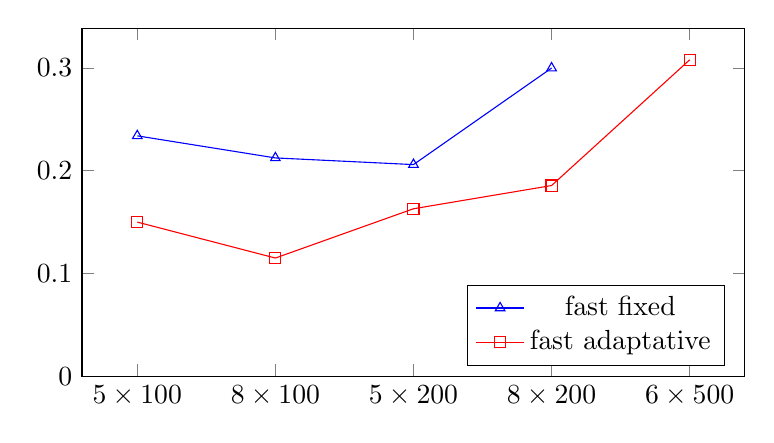
\begin{tikzpicture}
		\begin{axis}[width=10cm,height=6cm,
			xlabel={},
			ylabel={},
			legend pos=south east,
			ymin=0,
			xtick={1,2,3,4,5}, 
			xticklabels={$5\times 100$, $8\times 100$, $5\times 200$, $8\times 200$, $6\times 500$},
			]
			
			
			\addplot[mark=triangle, blue] coordinates {
				(1, 0.234)
				(2, 0.2125)
				(3, 0.206)
				(4, 0.3)
			};
			\addlegendentry{fast fixed}
			
			
			\addplot[mark=square, red] coordinates {
				(1, 0.15)
				(2, 0.115)
				(3, 0.163)
				(4, 0.1856)
				(5, 0.308)
			};
			\addlegendentry{fast adaptative}
			
			
		\end{axis}
	\end{tikzpicture}
	\caption{runtime (seconds per node)}
	\label{fig2}
\end{figure}



We now focus on understanding the potential of {\toolname} for even larger networks than those that are usually considered in the verification community. To this end, Figure~\ref{fig2} presents the  average runtime per node across various DNNS. Observe that while  the average runtime per node isn't fixed (attributable to $\LP(N,K)$), it remains regulated, avoiding exponential increases — from 0.1s per node for the smallest DNN to 0.3s per node for the largest. This suggests that {\toolname} is scalable to larger DNNs, bypassing the high complexity barrier often encountered with approaches such as those based on pure branch and bound.

\fi


\section{Discussion}
\label{Discussion}


In this work, we focused on DNNs employing ReLU activation functions since our approached on usage of MILP, which is naturally suited for ReLU activation function. However, it is worth remarking that the notion of compensation strength is independent of  activation function, and therefore, an interesting direction of future work would be to explore other the impact of compensation strength-based approaches for other activation functions. 


Regarding accuracy, {\toolname} ranks highly among verifiers that abstract values. However, its runtime, particularly for larger DNNs, can be relatively slow, though not excessively so. Numerous optimization avenues exist. A primary strategy involves utilizing $\alpha$-$\beta$-CROWN initially in the sequence, reserving {\toolname} for images unresolved by $\alpha$-$\beta$-CROWN, potentially enhancing this with parallel node computation across additional CPU cores. Another tactic could involve adapting the refined branch-and-bound approach of $\beta$-CROWN to permit {\toolname} to process additional layers beyond MILP's capability, concluding the verification with BaB. More complex strategies might include modifying BaB to branch on unstable ReLU nodes, driven by compensation strength, or analyzing crucial nodes linked to uncertain outputs, enabling quicker computation of less precise bounds for less critical nodes. Furthermore, implementing a Refinement Abstraction framework, akin to methodologies in \cite{atva}, \cite{elboher}, or \cite{SRGR}, could be beneficial.


In terms of neuron correlation, a key feature explicitly encoded by PRIMA, our findings suggest that leveraging compensation strength for network abstraction is generally more effective. Although precise local accuracy is achieved by directly considering ReLU nodes, the accuracy diminishes when correlations originate from distant layers. Retaining a select few significant correlations, in the style of PRIMA, as explicit linear constraints in the MILP model, might offer a strategy to further improve accuracy. 




%\section{Lipschitz}

We will introduce some formulas.




\section{Conclusion}
In this paper, we developed a novel solution-aware scoring (SAS) function to select few ReLU nodes to consider with binary variables to compute accurately bounds in DNNs. 
The solution awareness allows SAS to compute an accurate score for each ReLU, which enables partial MILP to be very efficient, necessitating $\approx6$x less binary variables than previous proposals \cite{DivideAndSlide} for the same accuracy. As the worst-case complexity is exponential in the number of binary variables, this big leap ahead has large implication in terms of scalability to larger DNNs, making it possible to verify quite large DNNs such as CNN-B-Adv with 2M parameters and 20000 activation functions. 

While $\alpha,\beta$-Crown is known to be extremely efficient to solve easier verification instances, we exhibit many cases (complex instances) where its worst-case exponential complexity in the number of ReLUs is tangible, with unfavorable scaling (Table \ref{table_beta}). Resorting to Hybrid MILP, a divide-and-conquer approach \cite{DivideAndSlide}, revisited thanks to the very efficient solution-aware scoring, revealed to be a much better trade-off than augmenting $\alpha,\beta$-Crown time-outs, with $8\%$ to $40\%$ less undecided images at ISO runtime.

Last, we adapted BaB-SR \cite{BaB} and FSB \cite{FSB} as global scoring (GS) functions. 
We compared GS with SAS both theoretically and experimentally with solution-aware scoring: While GS are not as efficient as SAS for ReLU {\em selection} (2x more binary variables needed), GS functions generate {\em static order} more adapted to every branch of a BaB process. This opens up interesting future research directions, to hybridize different scoring for different tasks;  e.g. verifying global \cite{lipshitz}, \cite{sensing} rather than local (robustness) properties.


%{\bf Reproducibility Statement:} We tested twice outlier results to confirm them, making sure of reproducibility on the given hardware. Precise details on the settings used are provided in the appendix. Additional results {\color{blue}(e.g. ablation studies)} are also provided in the appendix. Tested DNNs as well as MNIST and CIFAR10 DataSet are freely available. The source code of Hybrid MILP will be provided on GitHub after acceptance (needing Gurobi as well as $\alpha,\beta$-Crown).



\newpage


\bibliography{references}
\bibliographystyle{plain}


\bigskip

\appendix

\vspace{-0.6cm}

\section*{Appendix}

{\color{blue}
\section{Parameter settings}

\subsection*{Setting for $\alpha,\beta$-Crown}

The networks were already tested by $\alpha,\beta$-Crown \cite{crown}. We thus simply reused the parameter files from \href{https://github.com/Verified-Intelligence/alpha-beta-CROWN/blob/main/complete_verifier/exp_configs/beta_crown/}{their Github}, 
except for time-out which we explicitly mention.

e.g., for CNN-B-Adv: "solver: batch size: 512 beta-crown: iteration: 20" and
for MNIST 5x100: "solver: batch size: 1024 beta-crown: iteration: 20".

We did not experiment with cutting planes (GCP-CROWN \cite{cutting}), as it needs an additional package, namely IBM CPLEX solver, we do not have access to. From \cite{cutting}, the number of undecided inputs of GCP-CROWN is $\leq 2\%$ better than $\alpha,\beta$-Crown on the DNNs we experimented with, far from the $10-40\%$ improvement seen from Hybrid MILP. The conclusion are thus unchanged.
}

\subsection*{Setting for Hybrid MILP}


Hybird MILP first call $\alpha,\beta$-Crown with short time-out (TO), then call partial MILP on those inputs which was neither certified nor falsified by this run of $\alpha,\beta$-Crown. We are using two settings of TO, for smaller DNNs we use T0$=10s$, and for the two larger ones, we use TO$=30s$.

The setting for partial MILP for fully-connected DNNs is about how many neurons need to be opened (once set, the selection is automatic). The runtime depending crucially upon the number of open ReLU neurons, we set it quite tightly, only allowing few neuron deviation to accommodate to a particularly accurate/inaccurate bound computation (measure by the weight of the remaining Utility function). As complexity increases with the layer considered, as the size of the MILP model grows, we lower this number with the depth, only committing to an intermediate number for the output neuron (the number of output neurons  is smaller than hidden layer, and this is the most important computation). We experimentally set this number so that each computing the bounds in each hidden layer takes around the same time. Remember that in layer 1, partial MILP is not necessary and propagating bounds using interval arithmetic is already exact. We open [48,48] to compute bounds for hidden layer 2, [21,24] for layer 3, [11,14] for layer 4, [6,9] for layer 5, [3,6] for layer 6, [2,5] for layer 7, [1,4] for hidden layer 8 (if any), and we open [14,17] for the output layer.
{\color{blue} The exact number of open nodes in the range [a,a+3] is decided automatically for each neuron being computed : ReLUs are ranked according to their value by Utility, and the a top ReLUs are open. Then, ReLUs ranked a+1,a+2, a+3 are opened if their Utility value is larger than a small threshold. We set the threshold at 0.01. It should be seen as a way to save runtime when Utility knows that the next node by ranking (a+i) will not impact accuracy much (thanks to the upper bound from Proposition \ref{prop2}).}

\begin{table}[b!]
	\centering
	\begin{tabular}{||l||c|c||}
		\hline \hline
		Network & TO for $\alpha,\beta$-Crown  & Minimum number of Open neurons  \\ 		  
		\hline
		MNIST $5 \times 100$ & 10s  & 48,21,11,6,14  \\ \hline
		MNIST $5 \times 200$ & 10s & 48,21,11,6,14  \\ \hline
		MNIST $8 \times 100$ & 10s  & 48,21,11,6,3,2,1,14  \\ \hline
		MNIST $8 \times 200$ & 10s & 48,21,11,6,3,2,1,14  \\ \hline
		MNIST $6 \times 500$ & 30s & 48,21,11,6,3,14 \\ \hline
		CIFAR CNN-B-adv & 30s & 200, 0, 45 \\ \hline \hline
	\end{tabular}
	\caption{Settings of Hybrid MILP for the different {\em hard} instances}
	\label{table20}
	\end{table}


For convolutional CNNs, the strategy is adapted, as there is much more neurons, but in a shallower architecture and not fully connected. 
The second layer is computed accurately, opening 200 neurons, which is manageable as there is only one ReLU layer to consider, and accuracy here is crucial.
We do not open any nodes in the third layer (the first fully connected layer) if the output layer is the next one (which is the case for CNN-B-Adv), and instead rely on the choice of important nodes for the output layer. Otherwise, we open 20 neurons.
In the output layer, we open at least 45 neurons (there is less output neurons than nodes in the previous layer), and enlarge the number of open neurons (up to 300) till we find an upper bound, that is a best current MILP solution, of around +0.1 (this 0.1 was experimentally set as target, a good balance between accuracy and efficiency), and compute a guaranteed lower bound (the goal is to guarantee the bound is $>0$).

In Table \ref{table20}, we sum-up the TO and minimum open numbers for each DNN considered.

{\color{blue}
$\alpha,\beta$-Crown uses massively parallel ($>$4096 threads) GPU, while Partial MILP uses 20 CPU-threads.}

Notice that a different balance between accuracy and runtime could be set. For instance, we set up the numbers of open neurons to have similar runtime as Refined $\beta$-Crown for the first 4 DNNs ($50s-100s$). We could easily target better accuracy (e.g. for $8 \times 100$ with a relatively high $15\%$ undecided images) by increasing the number of open neurons, with a trade-off on runtime (current runtime is at $61s$).
By comparison, the sweet spot for $\alpha,\beta$-Crown seems to be around TO$=30s$, enlarging the time-out having very little impact on accuracy but large impact on runtime
(Table \ref{table_beta}).


{\color{blue}
Last, for Gurobi, we use a custom MIP-Gap (from $0.001$ to $0.1$) and time-out parameters, depending on the seen improvement and the possibility to make a node stable. This is low level implementation details that will be available in the code once the paper is accepted.
}





{\color{blue}

\section{Pseudocode and Complexity Analysis}	

\SetKwInput{KwInput}{Input}
\SetKwInput{KwOutput}{Output}

\begin{algorithm}[h!]
	\caption{pMILP($K$)}
	\label{algo1}
	\KwInput{Bounds $[\alpha_n,\beta_n]$ for input nodes $n$ at layer $0$ (input neighbourhood)}
	
	\KwOutput{Bounds $[\alpha_n,\beta_n]$ for every node $n$}
	
	\For{layer $k=1 \cdots \ell$}{
		\For{neuron $n$ in layer $k$}{
			
			Compute $X$ a set of $K$ nodes with the highest Utility for target neuron $n$.
			
			Run MILP$_X$ to obtain $[\alpha_n,\beta_n]$ from bounds of neurons in layers $< k$
		}
	}
\end{algorithm}	

%We then analyse its complexity.
%First, notice that the complexity to rnu Utility is negligible wrt the Run MILP$_X$.

We provide the pseudo code for pMILP in Algorithm \ref{algo1}.
pMILP($K$) has a worst case complexity bounded by $O(N \cdot \MILP(N,K))$, 
where $N$ is the number of nodes of the DNN, and $\MILP(N,K)$ is the complexity of solving a MILP program with $K$ integer variables and $N$ linear variables.
We have $\MILP(N,K) \leq 2^K \LP(N)$ where $\LP(N)$ is the Polynomial time to solve a Linear Program with $N$ variables, $2^K$ being an upper bound. Solvers like Gurobi are quite adept and usually do not need to evaluate all $2^K$ ReLU configurations to deduce the bounds.
It is worth mentioning that the "for" loop iterating over neurons $n$ in layer $k$ (line 2) can be executed in parallel, because the computation only depends on bounds from preceding layers, not the current layer $k$. 
%This parallelization results in a time complexity of $O(\sum_{i=1}^{\ell} \MILP(N_{i-1},K))$, where $\ell$ denotes the total number of layers and $N_i$ the count of neurons in layers $0, ..., i$. 
%pMILP uses 20 threads.


If $K$ is sufficiently small, 
%Algorithm \ref{algo1} invokes many MILP (e.g., using Gurobi) with a manageable number of %integer variables. 
this approach is expected to be efficient. 
The crucial part is thus to find few neurons which are particularly important when computing neuron $n$. This is where our novel Utility function outperforms previous solutions, by using an call to an (LP) solver to obtain a solution, which is novel as far as we know. This solutions allows to optimizing the choice of open nodes for the particular input considers, and appears significantly better than previous attempts, explaining the efficiency of the method.

For comparison, refined $\beta$-Crown and refined Prima used all the nodes up to a certain layer as binary variables, which is particularly inefficient, see Table \ref{table12} and Fig. \ref{fig4}. Hence, it can only be applied to small DNNs (it is implemented only up to MNNIST 8x200), while pMILP scales to at least 20.000 neurons (CNN-B-Adv).
\cite{DivideAndSlide} is the closest to pMILP, also implementing a choice of nodes as binary variables. However, their choice is particularly inefficient, as revealed by Table  
\ref{tab:example1}, needing 4 times the number of open nodes for the same accuracy as our Utility function.




\section{Ablation studies}	

In this section, we consider ablation studies to understand how each feature enables the efficiency of pMILP.

\subsection*{Time scaling with open nodes}	

First, we explore the time scaling with different number of open nodes, for our full Utility function using nodes in the last two layers (Layer 1 and 2), providing finer details than in Table 3, with the same setting, i.e. previous layer being computed with full MILP.





\begin{table}[h!]
		\centering
		\hspace*{4ex}
		\begin{subtable}[b]{0.45\textwidth}
		\begin{tabular}{|c|c|c|}
		\hline
		$|X|$ & Time & Uncertainty\\ 
		\hline	0 & 2.6 & 1.760946128\\
		\hline	1 & 7.3 & 1.702986873\\
		\hline	2 & 11.1 & 1.65469034\\
		\hline	3 & 16.3 & 1.612137282\\
		\hline	4 & 15.5 & 1.571001109\\
		\hline	5 & 15.7 & 1.531925404\\
		\hline	6 & 15.8 & 1.49535638\\
		\hline	7 & 16.4 & 1.46189314\\
		\hline	8 &  15.8 & 1.4299535\\
		\hline	9 &  17.2 & 1.4006364\\
		\hline	10 & 22.5 & 1.3711203\\
		\hline	11 & 27.2 & 1.3438245\\
		\hline	12 & 21.6 & 1.3183356\\
		\hline	13 & 28.7 & 1.2938690\\
		\hline	14 & 29.6 & 1.2690507\\
		\hline	15 & 24.5 & 1.2475106\\
		\hline
	  \end{tabular}
	\end{subtable}
	\hfill
	\begin{subtable}[b]{0.45\textwidth}
		\begin{tabular}{|c|c|c|}
			\hline
			$|X|$ & Time & Uncertainty\\ 
		\hline	16 & 31.9 & 1.2243065\\
		\hline	17 & 28.6 & 1.2031791\\
		\hline	18 & 30.4 & 1.1839474\\
		\hline	19 & 34.0 & 1.1644653\\
		\hline	20 & 42.1 & 1.1456181\\
		\hline	21 & 47.6 & 1.1261252\\
		\hline	22 & 62.7 & 1.1089745\\
		\hline	23 & 70.0 & 1.0931242\\
		\hline	24 & 70.8 & 1.0773088\\
		\hline	25 & 139.9 & 1.060928\\
		\hline	26 & 154.2 & 1.045715\\
		\hline	27 & 213.1 & 1.030605 \\
		\hline	28 & 211.3 & 1.016058\\
		\hline	29 & 373.1 & 1.001374\\
		\hline max=116 & 3300 & 0.895\\ 
		\hline		
	  \end{tabular}
     \end{subtable}
	  \caption{Time and uncertainty scaling of pMILP with number of nodes.}
    	\label{table14}
\end{table}


\begin{figure}[b!]
	\hspace*{-0.8cm}
	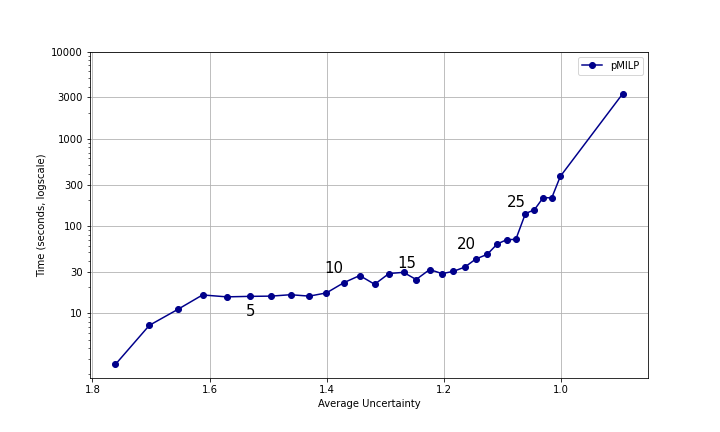
\includegraphics[scale=0.6]{Layer3_comparison}.
	\caption{Time and uncertainty scaling of pMILP with number of nodes.
	Time is using logscale.}
	\label{fig3}
\end{figure}


The exponential complexity with the number of nodes can be seen on Figure \ref{fig3}, where time is represented using logarithmic scale. The flat area in the middle is Gurobi having good heuristic to avoid considering all $2^K$ cases when $K<21$ is not too large, but not working so well for $K>25$. Notice that when certifying, pMILP uses $|X| \in$ 21-24, which is a good trade off between time and accuracy.


We also provide in Table \ref{tab:example1} the raw numbers used to produce Figure \ref{fig_table3}.
Further, we tested with the SR and FSB heuristics \cite{BaB}, that chooses nodes to branch on for BaB (Branch and Bound). When used instead to open nodes for pMILP, SR and FSB result in particularly low accuracy:
even though SR, FSB and \cite{DivideAndSlide} heuristic are all choosing ReLUs based on sensitivity of the target neuron $z$, SR and FSB are worse than \cite{DivideAndSlide} which only opens neurons one layer before (except when all ReLUs of the previous layers are open), and far worse than Utility. Further, FSB is performing worse than SR when choosing nodes for pMILP, while to choose nodes to branch on for BaB, it is the opposite. This likely means that the heuristic to choose nodes to branch for BaB is not adapted to choose nodes to open for pMILP.

\begin{table}[h!]	
	\centering
	\begin{tabular}{|c||c|c|c||c|c|c|c|}
		\hline
			&\multicolumn{3}{c||}{$X \subseteq$ Layer 2, max $=55$}&\multicolumn{4}{c|}{$X \subseteq$ Layers 1\&2, max $=116$} \\\cline{2-8}
		\text{$|X|$}  & \text{Random} & Huang & \bf Utility& \text{Random} & SR & FSB &\bf Utility\\ \hline
		\hline
		0  (LP) &   1.761  &1.761& 1.761 & 1.761  &  1.761& 1.761 & 1.761\\ \hline \hline
		5  &   1.729&1.704 & 1.603&  1.729& 1.7133 & 1.7149 & \bf 1.532 \\ \hline
		10  &  1.701 &  1.651 &1.517& 1.696 & 1.6674& 1.6714 & \bf  1.371\\ \hline
		15  & 1.671 &  1.599 &1.466&  1.653& 1.6230& 1.6251 & \bf  1.247\\ \hline
		20  &  1.635 & 1.557&1.438 & 1.619 &1.5764 & 1.5812 & \bf  1.145\\ \hline
		25  &  1.601 & 1.519 &1.427&  1.586 &1.5322 & 1.5388 & \bf 1.061\\ \hline
		30  & 1.574 & 1.489 &1.425& 1.546 &  1.4914& 1.4982 & \bf  0.989 \\ \hline
		35  &  1.542 & 1.465&1.424 & 1.502 & 1.4481 & 1.4600 & \bf 0.934 \\ \hline
		40  & 1.512 & 1.447 &1.424& 1.469 & 1.4070& 1.4187 & \bf 0.921 \\ \hline \hline
		max & 1.424  &1.424& 1.424 & 0.895 & 0.895 & 0.895 & 0.895   \\ \hline
	\end{tabular}
	\caption{Average uncertainty of $\MILP_X$ for nodes of the third layer, for $X$ with $K$ ReLU nodes of the (1st and) 2nd layer, chosen by our {\bf Utility} function vs \cite{ DivideAndSlide} vs SR vs FSB vs random choice.}
	\label{tab:example1}
	%\vspace{-0.6cm}
\end{table}



	\begin{figure}[h!]
		\centering
		\vspace*{-0.3cm}
		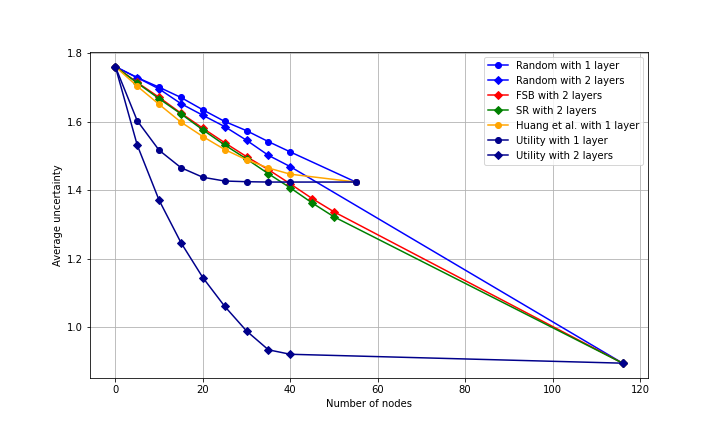
\includegraphics[height=9cm]{New Plot for table 3}.
		\vspace*{-0.4cm}
		\caption{Average uncertainty of $\MILP_X$ for nodes of the third layer, with ReLU nodes of the (1st and) 2nd layer, chosen by our {\bf Utility} function vs \cite{DivideAndSlide} vs vs SR vs FSB vs random.}
		\label{fig_table3_new}
	\end{figure}




\newpage

\subsubsection*{Usefulness of computing previous layers accurately}	


Then, we explore the usefulness of computing accurately each layer inductively.
For that, we keep the setting of Figure \ref{fig3} / Table \ref{table14}, but computing the previous layer with LP rather than with full MILP.


\begin{figure}[h!]
	\hspace*{-0.8cm}
	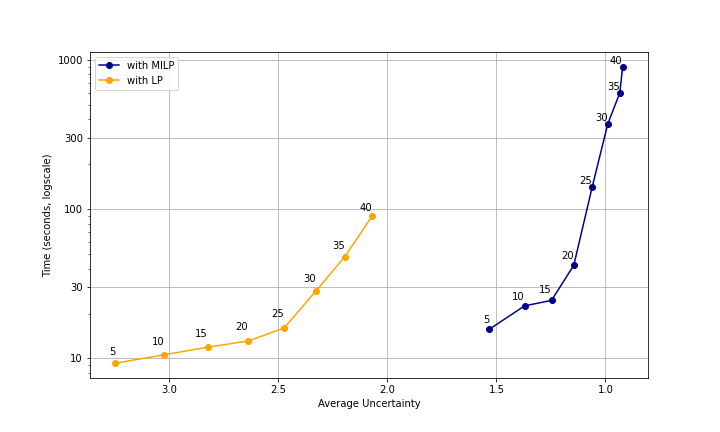
\includegraphics[scale=0.6]{Layer3_comparison_LP}.
	\caption{Comparison of accuracy in layer 3 when layer 2 is computed inaccurately using LP vs when layer 2 computed accurately using MILP.
	Time is using logscale.}
	\label{fig3LP}
\end{figure}








\begin{table}[h!]
	\centering
\begin{tabular}{|c|c|c|c|}
	\hline
	$|X|$ & Time &  With LP for layer 2 & With MILP for layer 2 \\ 
	\hline	5 & 9.3 & 3.24737  &1.532\\
	\hline	10 & 10.6 & 3.02214 & 1.371\\
	\hline	15 & 11.9 & 2.82383  &1.247\\
	\hline	20 & 13.1 & 2.63862 & 1.145\\
	\hline	25 & 16.0 & 2.47324 & 1.061\\
	\hline	30 & 28.3 & 2.32793  &0.989\\
	\hline	35 & 48.1 & 2.19506 & 0.934\\
	\hline	40 & 89.4 & 2.07107 & 0.921\\	
	\hline	
\end{tabular}
\caption{Comparison of accuracy in layer 3 when layer 2 is computed inaccurately using LP vs when layer 2 computed accurately using MILP.}
\label{table15}
\end{table}



This experiment explains the rationale to use divide and conquer protocol, using many calls
(one for each neuron) with relatively small number $|X|$ of open nodes rather than fewer calls to MILP with larger number $|X|$ of open nodes. This is clear already with only 1 layer before.


	
%		\begin{figure}[h]\hspace*{-1cm}
%		\includegraphics[scale=0.6]{Layzr3_comparison.png}.
%		\caption{Comparison of layer3 when layer 1 is MILP or LP}
%\label{fig4}
%	\end{figure}


\newpage

\subsubsection*{restricting number of open nodes (pMILP) vs setting time-outs (full MILP)}	

Running full MILP till a small MIP-Gap (typically 0.001) is reached is extremely time inefficient.

Instead, the standard strategy is to set a reasonable time-out and use whatever bound has been generated. We compare this standard strategy with the pMILP strategy of setting a priori a number of open nodes.

\begin{figure}[h!]\hspace*{-0.8cm}
	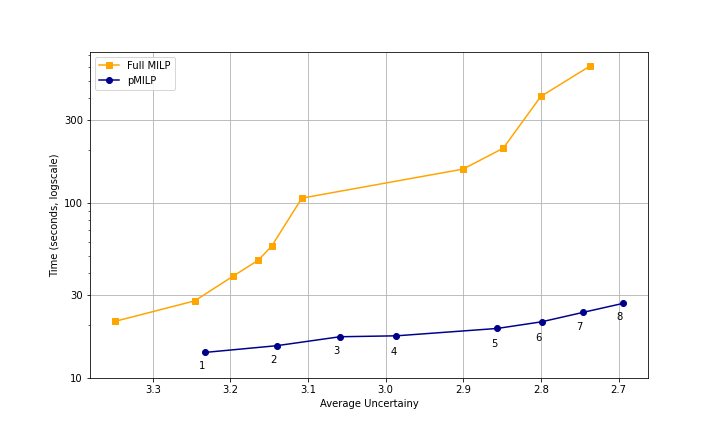
\includegraphics[scale=0.6]{Layer7_comparison.png}.
	\caption{Comparison of uncertainty at layer 7 for full MILP with different time-outs vs pMILP with different number of open nodes. Time is using logscale.}
	\label{fig4}
\end{figure}



\begin{table}[h!]
	\centering
	\hspace*{4ex}
\begin{subtable}[b]{0.45\textwidth}
	\centering
		\begin{tabular}{|c|c|c|}
	\hline
		$|X|$ & Time & Uncertainty\\ 
	\hline1 &	14 & 3.233021901\\
\hline	2 & 15.2 & 3.140309921\\
\hline	3 & 17.21 & 3.059083103\\
\hline 4 &	17.4 & 2.986166762\\
\hline	5 &19.2 & 2.856229765\\
\hline	6 &20.9 & 2.799248232\\
\hline	7 &23.7 & 2.746167245\\
\hline	8 &26.6 & 2.69485246\\	
	\hline
	\end{tabular}
	\caption{pMILP}
\end{subtable}
\hfill
\begin{subtable}[b]{0.45\textwidth}
	\centering
		\begin{tabular}{|c|c|}
		\hline
		Time & Uncertainty\\ 
		\hline	21.1 & 3.348236261\\
		\hline	27.6 & 3.24604282\\
		\hline	38.2 & 3.196640184\\
		\hline	47.1 & 3.164298172\\
		\hline	56.7 & 3.146913614\\
		\hline	106.7 & 3.108035223\\
		\hline	156.3 & 2.900438725\\
		\hline	205.8 & 2.848648426\\	
		\hline	406.7 & 2.800268264 \\	
		\hline	606.1 & 2.737064255\\	
		\hline
	\end{tabular}
		\caption{full MILP}
\end{subtable}
	\caption{Comparison of bounding the number of nodes for pMILP and 
	using different time outs for full MILP. In both settings, lower and upper bounds of previous layers are the same (computed by pMILP).}
	\label{table12}
	\end{table}

	

	

pMILP obtains 2.8 accuracy in $<21$ seconds (with 7 open nodes), while full MILP needs 400 seconds to obtain it, a 19x speed up. For 2.7 accuracy, the speedup is $>>$ 22.



Figure \ref{fig4} shows that choosing nodes is much more efficient for time/accuracy trade-off than setting time outs and use full MILP. And this is for the smallest DNN we considered (500 hidden neurons, far from the biggest 20k neuron DNN we experimented with)


\section{Comparison with other DNN verifiers}

In the following, we provide results comparing $\alpha,\beta$-Crown to other verifiers, to justify our use of $\alpha,\beta$-Crown as state of the art for efficient verifiers as main source of comparison to Hybrid MILP for hard DNN instance.


\subsection*{Comparison $\alpha,\beta$-Crown vs PRIMA}


\begin{table}[b!]
	\centering
	\begin{tabular}{||l||c|c||c||}
		\hline \hline
		Network & $\alpha,\beta$-Crown & Refined $\beta$-Crown & PRIMA \\ 		  
		\hline
		MNIST $5 \times 100$ & N/A  & 14.3\% (102s) & 33.2\% (159s)\\ \hline
		MNIST $5 \times 200$ & N/A & 13.7\% (86s) & 21.1\% (224s) \\ \hline
		MNIST $8 \times 100$ & N/A  & 20.0\% (103s) & 39.2\% (301s)   \\ \hline
		MNIST $8 \times 200$ & N/A & 17.6\% (95s) & 28.7\% (395s)  \\ \hline
		MNIST $6 \times 500$ & 51\% (16s) & $-$ & 64\% (117s) \\ \hline
		CIFAR CNN-B-adv & 18.5\% (32s) & $-$ & 27\% (344s)\\ \hline \hline
		CIFAR ResNet & 0\% (2s) & $-$ & 0\% (2s) \\ \hline \hline
	\end{tabular}
	\caption{Undecided images ($\%$, {\em lower is better}), as computed by $\alpha,\beta$-Crown, Refined $\beta$-Crown, and PRIMA, as reported in \cite{crown}, except for $6 \times 500$ that we run ourselves. N/A means that \cite{crown} did not report the numbers, while $-$ means that Refined $\beta$-Crown cannot be run on these DNNs.}
	\label{table9}
	%\begin{tablenotes}
	%	\footnotesize
%		\item Most data is directly from \cite{crown}. N/A means no data either in \cite{crown} or by our running.
%		\item  $^*$ The data in this row is from our own running on first 100 images of the MNIST dataset.
%		\item  $^{**}$ The data is from \cite{crown} on first 200 images of the CIFAR10 dataset.
%	\end{tablenotes}
	\end{table}


	PRIMA \cite{prima} is a major verifier in the ERAN toolkit. In Table \ref{table9}, we report the comparison between PRIMA and $\alpha,\beta$-Crown, mainly from \cite{crown}. The setting is mainly similar from ours, but numbers are not perfectly comparable as the images tested are not  exactly the same (1000 first or 200 first images for CNN-B-Adv), vs 100 first in Tables \ref{table_hybrid}, \ref{table_beta}. Also, time-out settings and hardware are slightly different. The overall picture is anyway the same.


Analysis: On the 4 smallest MNIST networks, PRIMA uses a refined path comparable with Refined $\beta$-Crown. However, it is slower and less accurate than Refined $\beta$-Crown.
On larger {\em hard} networks, PRIMA has also more undecided images than $\alpha,\beta$-Crown, while the runtime is $>5$ times larger.
Hence, Hybrid MILP is more accurate than Prima with similar runtime or faster.

Notice that kPoly \cite{kpoly}, OptC2V \cite{optC2V}, SDP-FO \cite{SDPFI} numbers were also reported in \cite{crown} on these networks, with even more unfavorable results.

\subsection*{Comparison $\alpha,\beta$-Crown vs MN-BaB}

MN-BaB \cite{ferrari2022complete} is an improvement built over PRIMA, using a similar Branch and Bound technique as used in $\alpha,\beta$-Crown. Results in \cite{ferrari2022complete}
are close to those of $\alpha,\beta$-Crown. However, none of the {\em hard} networks from \cite{crown} that we consider have been tested. We thus tested three representative {\em hard} DNNs (first 100 images) to understand how MN-BaB fairs on such hard instances, and report the numbers in Table \ref{table10}. Results are directly comparable with Table \ref{table_hybrid}.


\begin{table}[h!]
	\centering
	\begin{tabular}{||l||c|c||c|c||}
		\hline \hline
		 & $\alpha,\beta$-Crown & $\alpha,\beta$-Crown & MN-BaB & MN-BaB \\ 
		 Network & TO=30s & TO=2000s &  TO=30s & TO=2000s \\ 
		\hline
		MNIST $5 \times 100$ & 55\% (19s) & 50\%(1026s) & 60\% (19s) & 50\% (1027s) \\ \hline
		MNIST $6 \times 500$ & 51\% (16s) & 50\% (1002s) & 58\% (18s) & 55\% (1036s) \\ \hline
		CIFAR CNN-B-adv & 22\% (8.7s) & 20\% (373s) & 43\% (14s) & 24\% (576s) \\ \hline 
	\end{tabular}
	\caption{Undecided images ($\%$, {\em lower is better}), as computed by $\alpha,\beta$-Crown, and MN-BaB}
	\label{table10}
\end{table}

Analysis: results reveal that MN-BaB is slightly slower and slightly less accurate than $\alpha,\beta$-Crown. Notice the specially high number of undecided images for CNN-B-Adv with TO=30s, probably meaning that 30s is too small for MN-BaB on this large DNN.
Hence, Hybrid MILP is more accurate than MN-BaB with similar runtime or faster.



	\subsection*{Comparison $\alpha,\beta$-Crown vs NNenum}

NNenum \cite{nnenum} is a complete verifier with good performance according to VNNcomp.
It was the only complete verifier tested in Table \ref{table_complete} to verify more images than $\alpha,\beta$-Crown. The experiments section in \cite{nnenum} does not report
the {\em hard} DNNs we are considering. We tried to experiment it on the same MNIST 
$6 \times 500$ and CIFAR CNN-B-adv as we did in Table \ref{table10} for MN-BaB. Unfortunately, on $6 \times 500$, buffer overflow were reported.
We report in Table \ref{table11} experiments with the same 2000s Time-out (it was $10 000s$ in Table \ref{table_complete})  for a fair comparison with $\alpha,\beta$-Crown, on both 
MNIST $5 \times 100$ and CIFAR CNN-B-Adv. 
On MNIST $5 \times 100$, NNenum is slightly more accurate than $\alpha,\beta$-Crown, but far from the accuracy Hybrid MILP.
On CIFAR CNN-B-adv, NNenum was much less accurate than $\alpha,\beta$-CROWN, and thus of Hybrid MILP. In both test, the runtime of NNenum was also much longer than for Hybrid MILP.


\begin{table}[h!]
	\centering
	\begin{tabular}{||l||c||c||c||c||}
		\hline \hline
		 & $\alpha,\beta$-Crown & NNenum & Hybrid\\ 
		 Network & TO=2000s &  TO=2000s & MILP\\ 
		\hline
		MNIST $5 \times 100$ & 50\%(1026s) & 44\% (1046s) & \bf 13\% (46s)\\ \hline
		CIFAR CNN-B-adv & 20\% (373s) & 40\% (1020s) & \bf 11\% (417s)\\ \hline 
	\end{tabular}
	\caption{Undecided images ($\%$, {\em lower is better}), as computed by $\alpha,\beta$-Crown and NNenum with 2000s time-out, and Hybrid MILP}.
	\label{table11}
\end{table}


{\color{blue}

\section{Average vs max time per pMILP call}

We provide in Table \ref{table112} the average as well as maximum time to perform $MILP_X$ calls as called by pMILP, on a given input: image 3 for MNIST, and image 76 for CIFAR10. 
For 6x500, we provide results for two different $\varepsilon$, following our test from Figure \ref{fig2}.

\begin{table}[h!]
	\centering
	\begin{tabular}{||l|c|c||}
		\hline
		Network & average time & maximum time \\ \hline
		MNIST 5$\times$100 & 0.41s & 1.87 \\
		$\epsilon = 0.026$ &  & \\  \hline
		MNIST 5$\times$200 &  0.75s & 5.31s \\ 
		$\epsilon = 0.015$ & & \\  \hline
		MNIST 8$\times$100 & 0.39s & 1.41s \\
		$\epsilon = 0.026$ & &  \\  \hline
		MNIST 8$\times$200 & 0.49s & 1.63s \\ 
		$\epsilon = 0.015$ & & \\  \hline
		MNIST 6$\times$500 & &   \\ 
		$\epsilon = 0.035$ & 1.4s & 3.5s \\ 
		$\epsilon = 0.1$ & 44.6s & 310s \\  \hline 
		CIFAR CNN-B-adv &  & \\
		$\epsilon = 2/255$& 1s & 609s \\ \hline \hline
	\end{tabular}
	\caption{average and maximum time per $\MILP_X$ calls for image 3 (MNIST) and image 76 (CIFAR10).}
	\label{table112}
\end{table}

Notice that DNN 6$\times$ 500 and $\epsilon=0.1$ is a very hard instance as being very close to the falsification $\epsilon \approx 0.11$. This is thus not representative of the average case. Also,  on this image 3, pMILP succeeds to verify $\epsilon= 1.054$, while $\alpha,\beta$-CROWN can only certify $\epsilon = 0.0467$ within the 10 000s Time-out.

For CNN-B-Adv, the very long maximum time for a MILP call is an outlier: it happens only for one output layer, for which the number $K$ of open nodes is particularly large (around 200 out of 20000 neurons) to certify this hard image 76. Indeed, the average time is at $1s$. Notice that this does not lead to a runtime of 20.000s, as 20 threads are used by pMILP 
in parallel (similar to competing solutions, except $\alpha,\beta$-CROWN which uses $>4096$ GPU cores).


}









\end{document}


\section{SR Heuristic for choosing nodes}

Here we provide the formula of BaB-SR from paper \cite{BaB}.

\begin{align*}
	\nu_{n+1} &= -1&\\
	\hat{\nu}_k &= W^T_kv_{k+1}, k = n,\cdots,1 &\\
	\nu_{k,j} &= \begin{cases}
		0  &\text{ if }u_{k[j]}<0 \hspace*{2ex}(j\in\mathcal{I}^-_k)\\
		\hat{\nu}_{k[j]} &\text{ if }l_{k[j]}>0 \hspace*{2.5ex}(j\in\mathcal{I}^-_k)\\
		\frac{u_{k[j]}}{u_{k[j]}-l_{k[j]}}[\hat{\nu}_{k[j]}]_+-\frac{u_{k[j]}}{u_{k[j]}-l_{k[j]}}[\hat{\nu}_{k[j]}]_-  &\text{ otherwise } \hspace*{3ex}(j\in\mathcal{I}_k)\\ 
	\end{cases}\\
	&\hspace*{22ex}\text{for } k = n,\cdots,2&
\end{align*}and\begin{align*}
	s_{i[j]} = |\max(v_{i[j]}b_{i-1[j]},(v_{i[j]}-1)b_{i-1[j]})-\frac{u_{k[j]}}{u_{k[j]}-l_{k[j]}}[\hat{\nu}_{k[j]}]_+|
\end{align*}


\begin{figure}[b!]
	\hspace*{-0.8cm}
	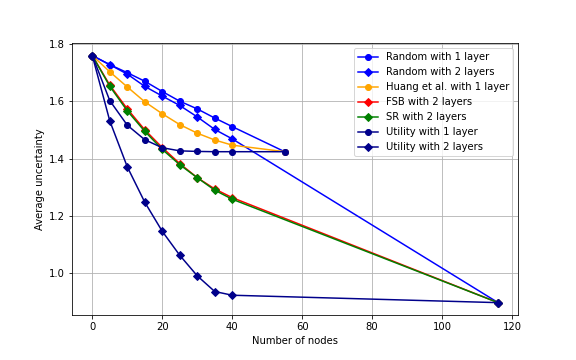
\includegraphics[scale=0.6]{Plot for table 3}.
	\caption{Plot for table 3}
	\label{fig_table3}
\end{figure}


\begin{table}[h!]	
	\centering
	\begin{tabular}{|c||c|c|c|c|}
		\hline
		&\multicolumn{3}{c|}{$X \subseteq$ Layers 1\&2, max $=116$}\\\cline{2-5}
		\text{$|X|$} & \text{Random} &BSR &FSB &\bf Utility\\ \hline
		0  (LP) & 1.761  &  1.761& 1.761&1.761\\ \hline \hline
		5  & 1.729& 1.7138 & 1.7182 &\bf 1.532 \\ \hline
		10  & 1.696 & 1.6775&  1.6803&\bf  1.371\\ \hline
		15  &   1.653& 1.6392& 1.6475&\bf  1.247\\ \hline
		20  &   1.619 &1.5938 & 1.6174&\bf  1.145\\ \hline
		25  &    1.586 &1.5534 &1.5788 &\bf 1.061\\ \hline
		30  &  1.546 & 1.5166& 1.5413&\bf  0.989 \\ \hline
		35  &   1.502 & 1.4788 &1.4972 &\bf 0.934 \\ \hline
		40  &  1.469 & 1.4395& 1.4514&\bf 0.921 \\ \hline \hline
		max &  0.895 & 0.895 &0.895 &0.895   \\ \hline
	\end{tabular}
	\caption{BSR and FSB}
	\label{BSRandFSB}
	%\vspace{-0.6cm}
\end{table}



\end{document}




\subsection*{Formula for ResNet}

Consider a ResNet, like ResNet4b, we list the formula for an Add layer.

Suppose we are dealing with an Add layer $l$, target node $z$, with previous layer $l_1$ and shortcut connection previous layer $l_2$, starting from a layer $l_0$, that is:
\begin{align*}
	l &= l_1+l_2\\
	l_2 &= Conv_{W_2}(\ReLU(l_0))\\
	l_1' &= Conv_{W'_1}(\ReLU(l_0))\\
	l_1 &= Conv_{W_1}(\ReLU(l'_{1}))
\end{align*}The paths are $$l_0\rightarrow \ReLU(l_0)\rightarrow l_2\rightarrow l,$$ and $$l_0\rightarrow \ReLU(l_0)\rightarrow l'_1\rightarrow \ReLU(l_1')\rightarrow l_1\rightarrow l.$$

So, for nodes in layer $l_1'$, we can use the same formula as previous section, i.e., the formula at the end of page 6: for a node $b$ in $l_1'$, suppose $z=x+y$ for $x$ in layer $l_1$ and $y$ in $l_2$, 
\begin{align*}
\Utility\_\max\nolimits^x(b) &= W_{bx} \times (\sol(\hat{b})- \ReLU(\sol(b)))\\
\Utility\_\max\nolimits^z(b) &= \Utility\_\max\nolimits^x(b)
\end{align*}

For nodes in layer $l_0$, the simple idea is to consider both paths, and sum up the utilities of two paths. For a node $a$ in $l_0$, suppose $z=x+y$ for $x$ in layer $l_1$ and $y$ in $l_2$ ,
\begin{align*}
		\Delta(\hat{a}) &= \ReLU(\sol(a))-\sol(\hat{a})\\
		\Utility_\_\max\nolimits^y(a) &= -W_{ay} \Delta(\hat{a})\\
	\forall b \in \ell, \Delta(b) &= W_{ab}\Delta(\hat{a})\\
	\forall b \in \ell, \Delta(\hat{b}) &=
	\begin{cases}
		\frac{\UB(b)}{\UB(b)-\LB(b)}\Delta(b),  &\text{if }W_{bx} > 0\\
		\max(\Delta(b),-\sol(b)),  &\text{if }  W_{bx} < 0 \text{ and } \sol(b)\geq0\\
		\max(\Delta(b)+\sol(b),0),  &\text{if }  W_{bx} < 0 \text{ and } \sol(b)<0		 
	\end{cases}\\
	\Utility\_\max\nolimits^x(a) &= -\sum_{b \in \ell} W_{bx} \Delta(\hat{b})\\
	\Utility\_\max\nolimits^z(a) &= \Utility\_\max\nolimits^x(a)+\Utility\_\max\nolimits^y(a)
\end{align*}

	
	
		
	


\section{Formula for Utility}


Recall that for nodes $a,b$, we use 
$\hat{a}, \hat{b}$ to denote variable after ReLU functions, and
$\Delta(a),\Delta(\hat{a}),\Delta(b),\Delta(\hat{b})$ to denote the changes of those variables. $a$ means the source node, and $b$ means nodes one layer after $a$, and $z$ is 2 layers after $a$ and one after $b$.

The utility function for a node $a$ wrt neuron $z$ is defined inductively as follows:


\begin{align*}
	\Delta(\hat{a}) &= \ReLU(\sol(a))-\sol(\hat{a})\\
	\Delta(b) &= W_{ab}\Delta(\hat{a})\\
	\Delta(\hat{b}) &=
	\begin{cases}
		\frac{\UB(b)}{\UB(b)-\LB(b)}\Delta(b),  &\text{if }W_{bz} > 0\\
		\max(\Delta(b),-\sol(b)),  &\text{if }  W_{bz} < 0 \text{ and } \sol(b)\geq0\\
		\max(\Delta(b)+\sol(b),0),  &\text{if }  W_{bz} < 0 \text{ and } \sol(b)<0		 
	\end{cases}\\
	\Utility\_\max\nolimits^z(a) &= -\sum_{b \in \ell} W_{bz} \Delta(\hat{b})
\end{align*}

}




\end{document}


